\documentclass[11pt,oneside]{book}

% =============================================================================
% Mass Spectrometry Data Analysis with R
% Chapter 19: Missing Data in Mass Spectrometry: Mechanisms, Imputation Theory, 
%              and Sensitivity Auditing
% Author: Lucas VHH TRAN (CK-CARE Davos)
% Style: Springer Nature Monograph (Health Analytics with R Pedagogy)
% =============================================================================

\usepackage{springer_monograph}

\hypersetup{
    pdftitle={Chapter 19: Missing Data in Mass Spectrometry: Mechanisms, Imputation Theory, and Sensitivity Auditing},
    pdfauthor={Lucas VHH TRAN}
}

\begin{document}

% --- Chapter Title Block ---
\setcounter{chapter}{18}
\chapter{Missing Data in Mass Spectrometry: Mechanisms, Imputation Theory, and Sensitivity Auditing}

\noindent
\textbf{Lucas VHH TRAN}\footnote{CK-CARE Davos, Christine K\"uhne -- Center for Allergy Research and Education, Davos, Switzerland. Email: \texttt{lucas.tran@ck-care.ch}}\\
\rule{\textwidth}{0.8pt}

\begin{abstract}
\noindent
Quantitative mass spectrometry datasets contain between 20\% and 50\% missing values~\cite{webb2020review, lazar2016accounting}. In clinical biomarker cohorts, this missingness presents an acute methodological problem: standard multivariate algorithms require complete matrices, yet the numerical substitution of missing values alters the variance structure, covariance relationships, and downstream statistical inferences of the entire dataset. Missingness in mass spectrometry does not arise from a single homogeneous process. A feature may be absent due to stochastic precursor selection during instrument duty cycles (Missing at Random; MAR), physical left-censoring below the instrument limit of detection (Missing Not at Random; MNAR), or true biological non-expression. Applying a MAR algorithm such as $k$-nearest neighbors to an MNAR peptide invents artificial intermediate abundances for molecules that were genuinely absent, while applying left-censored substitution to MAR values introduces downward bias and artificially inflates differential abundance discoveries. This chapter establishes the statistical, biophysical, and computational foundations required to diagnose, model, and impute missing data in mass spectrometry. We formalize Rubin's missing data taxonomy within an analytical chemistry context, analyze the mathematical properties of deterministic, stochastic, and machine-learning imputation algorithms, derive Rubin's pooling rules for multiple imputation with Barnard--Rubin small-sample degrees of freedom, and evaluate imputation-free probabilistic dropout modeling (\texttt{proDA}). The chapter concludes with a tutor diagnostic heuristics checklist, an end-to-end reproducible R laboratory, the Five Deadly Sins of omics imputation, and multi-tier exercises with worked solutions.
\end{abstract}

\noindent
\textbf{Keywords:}\enspace Missing Data, Imputation, Missing Not At Random (MNAR), Missing At Random (MAR), Left-Censoring, QRILC, Multiple Imputation, Rubin's Rules, Sensitivity Analysis, proDA.

\vspace{0.8em}
\noindent\rule{\textwidth}{0.4pt}

% =============================================================================
\section{Tutor's Methodological Roadmap for Missing Data Management}
% =============================================================================

Before applying imputation functions or running automated pipelines, the analytical chemist and biostatistician must diagnose the underlying missingness architecture. Table~\ref{tab:missing_roadmap} outlines the four sequential checkpoints required to handle missing data.

\begin{table}[htbp]
\centering
\caption{Tutor's Methodological Roadmap: Four Checkpoints for Missing Data Management}
\label{tab:missing_roadmap}
\small
\begin{tabularx}{\textwidth}{l p{3.8cm} p{4.2cm} X}
\toprule
\textbf{Stage} & \textbf{Physical Mechanism} & \textbf{Key Analytical Objective} & \textbf{Primary Failure Mode \& Remedy} \\
\midrule
\textbf{1. Diagnosis} & Instrumental left-censoring ($y < \text{LOD}$) vs. stochastic precursor selection \cite{rubin1976inference, lazar2016accounting}. & Fit logistic missingness curve (Eq.~\ref{eq:mnar_logistic}) to separate MNAR from MAR. & Misclassifying MNAR as MAR. Remedy: Test logistic slope $\gamma_1$; inspect intensity-dependent missingness \cite{ahlmann2020proda}. \\
\addlinespace
\textbf{2. Filtering} & Extreme feature sparsity across biological replicates \cite{webb2020review, karpievitch2012normalization}. & Enforce 70\% presence rule \textit{within at least one biological group}. & Filtering across entire cohort discards true on/off biomarkers. Remedy: Filter group-wise \cite{zhang2018dep}. \\
\addlinespace
\textbf{3. Modeling} & Tail-censored Gaussian draws vs. donor matching vs. probabilistic dropout \cite{tyanova2016perseus, ahlmann2020proda, palstrom2020imputation}. & Substitute missing values appropriately, or model dropouts directly without imputation. & Deterministic zero/min replacement spikes variance. Remedy: QRILC or proDA \cite{ahlmann2020proda}. \\
\addlinespace
\textbf{4. Sensitivity Audit} & Variance shrinkage underestimation from single imputation \cite{rubin1987multiple, little2019statistical}. & Quantify inferential stability across multiple imputation draws via Rubin's rules and evaluate covariance preservation via ADCS \cite{templ2023visualization}. & Downstream $p$-values falsely anti-conservative; distorted covariance. Remedy: Report multiple imputation pooled SE \cite{barnard1999small, vanbuuren2018} and audit NRMSE/ADCS \cite{templ2023visualization}. \\
\bottomrule
\end{tabularx}
\end{table}

\begin{notebox}
\textbf{Tutor's Note: The Rule of Group-Wise Filtering}\\
Never apply global missingness filters across an entire clinical cohort (e.g., ``remove all proteins with $>30\%$ missing values overall''). If a biomarker is abundant in Disease ($100\%$ detected in 10 patients) but silenced in Control ($0\%$ detected in 10 patients), global filtering eliminates this candidate ($10/20 = 50\% < 70\%$). Always require $\ge 70\%$ detection \textit{within at least one condition} \cite{zhang2018dep, webb2020review}.
\end{notebox}

% =============================================================================
\section{Biophysical Taxonomies of Missingness in Mass Spectrometry}
% =============================================================================

Donald Rubin~\cite{rubin1976inference} established the formal mathematical classification of missing data mechanisms based on the conditional distribution of the missingness indicator matrix.

\subsection{Rubin's Missing Data Taxonomy}

Let $\mathbf{Y} \in \mathbb{R}^{p \times n}$ denote the complete data matrix of $p$ molecular features across $n$ biological samples. We partition $\mathbf{Y} = (\mathbf{Y}_{\text{obs}}, \mathbf{Y}_{\text{mis}})$, where $\mathbf{Y}_{\text{obs}}$ represents observed quantitative intensities and $\mathbf{Y}_{\text{mis}}$ represents missing entries. Define the binary missingness response indicator matrix $\mathbf{M} \in \{0, 1\}^{p \times n}$ such that:
\begin{equation}
M_{ij} = \begin{cases} 1 & \text{if } y_{ij} \text{ is missing} \\ 0 & \text{if } y_{ij} \text{ is observed} \end{cases}
\end{equation}

The missing data mechanism is characterized by the conditional probability distribution $P(\mathbf{M} \mid \mathbf{Y}, \boldsymbol{\phi})$, parameterized by $\boldsymbol{\phi}$:

\begin{enumerate}
    \item \textbf{Missing Completely at Random (MCAR):} Missingness is independent of both observed and unobserved feature abundances:
    \begin{equation}
    P(\mathbf{M} \mid \mathbf{Y}_{\text{obs}}, \mathbf{Y}_{\text{mis}}, \boldsymbol{\phi}) = P(\mathbf{M} \mid \boldsymbol{\phi})
    \end{equation}
    In MS instrumentation, MCAR occurs during random electrospray droplet instabilities, momentary liquid chromatography pressure spikes, or random ion guide transmission dropouts.
    
    \item \textbf{Missing at Random (MAR):} Missingness depends systematically on observed data, but is conditionally independent of the unobserved missing value itself:
    \begin{equation}
    P(\mathbf{M} \mid \mathbf{Y}_{\text{obs}}, \mathbf{Y}_{\text{mis}}, \boldsymbol{\phi}) = P(\mathbf{M} \mid \mathbf{Y}_{\text{obs}}, \boldsymbol{\phi})
    \end{equation}
    In DDA mass spectrometry, precursor scheduling introduces dual mechanisms:
    (i) If a precursor ion is detected in the survey MS1 spectrum with known intensity, but fails to be scheduled for MS2 fragmentation due to the instrument top-$N$ duty cycle, missingness is conditional on the observed MS1 intensity and local chromatographic peak density, satisfying the MAR assumption~\cite{cox2014maxlfq}.
    (ii) Conversely, if a peptide is present at low concentration and fails to generate an MS1 signal above detector noise, missingness depends on its unobserved concentration, constituting true MNAR left-censoring~\cite{karpievitch2012normalization, lazar2016accounting}.
    
    \item \textbf{Missing Not at Random (MNAR):} Missingness depends directly on the unobserved value $\mathbf{Y}_{\text{mis}}$:
    \begin{equation}
    P(\mathbf{M} \mid \mathbf{Y}_{\text{obs}}, \mathbf{Y}_{\text{mis}}, \boldsymbol{\phi}) \ne P(\mathbf{M} \mid \mathbf{Y}_{\text{obs}}, \boldsymbol{\phi})
    \end{equation}
    This is the primary physical driver of missingness in analytical chemistry: analytes present below the instrument limit of detection (LOD) or limit of quantitation (LOQ) fail to generate a discernible chromatographic peak above baseline noise.
\end{enumerate}

\subsection{Compositional Data and Analytical Zero Taxonomies (Templ 2023)}

Mass spectrometry measurements are fundamentally relative: detector ion currents reflect proportional abundances within a finite total ion current (TIC) or sample loading. Following the compositional data framework established by John Aitchison~\cite{aitchison1986statistical} and Matthias Templ~\cite{templ2023visualization}, analytical chemistry distinguishes three distinct forms of unobserved or zero values:
\begin{enumerate}
    \item \textbf{Values Below Detection Limit (BDL) or Rounded Zeros:} Continuous chemical concentrations that fall below the physical sensitivity of the instrument ($y_{ij} < \text{LOD}$). This is the primary physical cause of left-censored MNAR in label-free proteomics.
    \item \textbf{Count Zeros:} Absolute absence of discrete ion detection events in integer count datasets (such as spectral counting or low-intensity tandem MS/MS transitions).
    \item \textbf{Structural Zeros:} Biological non-expression where the protein or metabolite is physically absent ($y_{ij} \equiv 0$). This occurs in tissue-specific gene silencing, knockout models, or non-synthesized secondary metabolites.
\end{enumerate}
Treating BDL values as structural zeros creates false biological silencing. Furthermore, while standard statistical workflows apply logarithmic transformation $\log_2(y_{ij})$ as an approximation to unconstrained Euclidean geometry, Templ~\cite{templ2023visualization} and Aitchison~\cite{aitchison1986statistical} demonstrate that value substitution on $\log$-intensities can perturb isometric log-ratios (ILR). Imputation methods that preserve relative covariance (such as regularized donor matching or model-based likelihoods) are required to avoid distorting downstream ratio-based network topology.

\subsection{Analytical Mechanisms in Proteomics and Metabolomics}

Proteomics and metabolomics experiments exhibit compound missingness patterns driven by instrument operation and experimental design:
\begin{itemize}
    \item \textbf{Data-Dependent Acquisition (DDA) Duty Cycles:} In shotgun proteomics, the instrument alternates between survey MS1 scans and data-dependent MS2 fragmentation scans of the top-$N$ most intense precursor ions. When chromatographic peak capacity is exceeded, lower-intensity co-eluting ions are bypassed, generating MAR dropouts \cite{cox2014maxlfq, julian2024rprogramming}.
    \item \textbf{Analytical Left-Censoring:} Analytes with low solution concentration or low ionization efficiency yield detector currents below the signal-to-noise threshold ($S/N < 3$), resulting in left-censored MNAR values \cite{karpievitch2012normalization, lazar2016accounting}.
    \item \textbf{Merged Cohorts and Isobaric Multiplexing:} In multi-batch isobaric labeling (TMT or iTRAQ) and large-scale label-free clinical studies, combining multiple LC-MS/MS runs compounds missingness. Features identified in one batch may fail identification in another due to run-to-run retention time drift or stochastic precursor selection \cite{palstrom2020imputation, mcalister2014multinotch}.
    \item \textbf{Biological Non-Expression (Structural Zeroes):} Proteins absent due to gene knockouts or tissue-specific expression are structural zeroes ($y_{ij} \equiv 0$). Imputing structural zeroes creates false molecular noise and distorts biological specificity.
\end{itemize}

\begin{pitfallbox}
\textbf{The Tissue-Atlas Imputation Catastrophe}\\
In multi-organ proteomics atlases (such as profiling 30 human tissues), a liver-specific enzyme absent in cardiac muscle is missing due to biological regulation, not instrument failure. Imputing this enzyme in cardiac samples using left-censored algorithms introduces false molecular noise and destroys biological specificity. Never impute structural biological absence \cite{lazar2016accounting}.
\end{pitfallbox}

\subsection{Mathematical Diagnosis of Missingness Mechanisms}

To diagnose whether a dataset is dominated by MAR or MNAR, we fit a logistic regression model linking feature missingness probability to its mean observed abundance:
\begin{equation}
\label{eq:mnar_logistic}
\operatorname{logit}\left( P(M_{ij} = 1 \mid \bar{y}_i^{\text{obs}}) \right) = \ln\left( \frac{P(M_{ij} = 1)}{1 - P(M_{ij} = 1)} \right) = \gamma_0 + \gamma_1 \bar{y}_i^{\text{obs}}
\end{equation}
where $\bar{y}_i^{\text{obs}} = \frac{1}{|O_i|}\sum_{j \in O_i} y_{ij}$ denotes the mean observed $\log_2$ intensity for feature $i$.
Because observed data alone cannot formally confirm MNAR without untestable assumptions on the unobserved conditional distribution~\cite{rubin1976inference, little2019statistical}, the logistic slope serves as an empirical diagnostic:
\begin{itemize}
    \item If $\gamma_1 < 0$ with statistical significance ($p < 0.001$), missingness increases as observed abundance decreases, providing empirical evidence consistent with \textbf{abundance-dependent MNAR left-censoring}.
    \item If $\gamma_1 \approx 0$ (a flat slope across the dynamic range), missingness is abundance-independent, consistent with \textbf{MAR or MCAR}.
\end{itemize}

Figure~\ref{fig:missingness_diagnosis} illustrates this empirical diagnosis on a 400-protein benchmark cohort.

\begin{figure}[htbp]
\centering
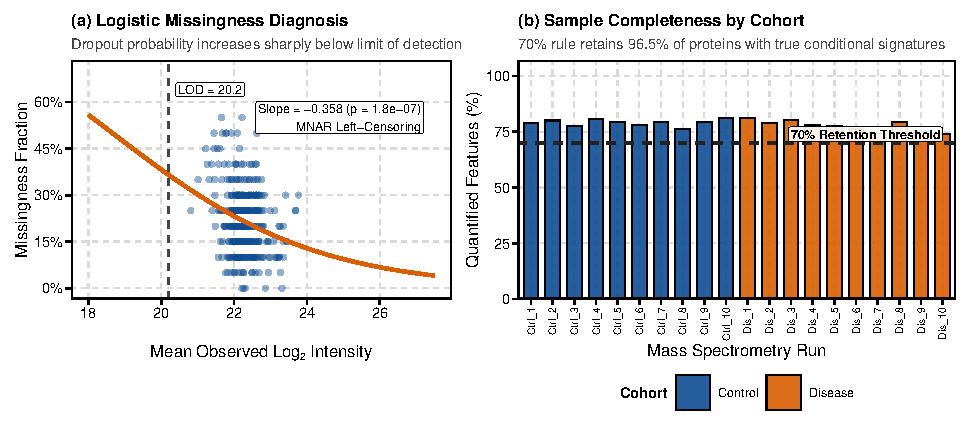
\includegraphics[width=\textwidth]{figures/fig_19_1_missingness_diagnosis.pdf}
\caption{Empirical diagnosis of missingness architecture and group-wise completeness. Panel A: Logistic missingness diagnosis curve modeling dropout probability as a function of mean observed abundance. The negative slope ($\hat{\gamma}_1 = -0.358$, $p = 1.78 \times 10^{-7}$) establishes abundance-dependent MNAR left-censoring below the limit of detection ($\text{LOD} = 20.2$). Panel B: Sample-by-sample feature completeness comparing Control and Disease cohorts, demonstrating that group-wise filtering ($\ge 70\%$ in $\ge 1$ group) preserves true on/off biomarkers.}
\label{fig:missingness_diagnosis}
\end{figure}

\subsection{Formal Hypothesis Testing: Little's Multivariate MCAR Test}

Beyond univariate logistic curves, Donald Rubin and Roderick Little~\cite{little1988test, templ2023visualization} established the multivariate omnibus test for Missing Completely at Random (MCAR). The sample of $n$ observations is partitioned into $S$ distinct missingness patterns, where pattern $s$ contains $n_s$ samples with an identical subset of $p_s$ observed variables. Little's test statistic evaluates the weighted sum of squared Mahalanobis distances between pattern-specific observed means $\bar{\mathbf{y}}_{\text{obs}, s}$ and maximum likelihood mean estimates $\hat{\boldsymbol{\mu}}_{\text{obs}, s}$ obtained via the Expectation-Maximization (EM) algorithm:
\begin{equation}
\label{eq:little_mcar}
d_{\text{MCAR}}^2 = \sum_{s=1}^S n_s \left( \bar{\mathbf{y}}_{\text{obs}, s} - \hat{\boldsymbol{\mu}}_{\text{obs}, s} \right)^T \hat{\boldsymbol{\Sigma}}_{\text{obs}, s}^{-1} \left( \bar{\mathbf{y}}_{\text{obs}, s} - \hat{\boldsymbol{\mu}}_{\text{obs}, s} \right)
\end{equation}
Under the null hypothesis that missingness is MCAR, $d_{\text{MCAR}}^2$ asymptotically follows a central $\chi^2$ distribution with $\sum_{s=1}^S p_s - p$ degrees of freedom~\cite{little1988test, templ2023visualization}.

Two critical methodological principles govern the interpretation of Little's test in mass spectrometry:
\begin{enumerate}
    \item \textbf{Inferential Scope:} Rejection of the null hypothesis ($p < 0.05$) establishes that data are \textit{not} MCAR; this rejection is compatible with either MAR or MNAR and cannot distinguish between them.
    \item \textbf{High-Dimensionality ($p > n$):} Little's test requires inverting the observed-data covariance matrix $\hat{\boldsymbol{\Sigma}}_{\text{obs}, s}$, which becomes singular when features exceed sample size ($p > n$). The test can therefore only be computed on representative low-dimensional blocks ($p < n$). As demonstrated in Section~\ref{sec:r_laboratory}, on a small 6-protein subset ($n=20$), the test statistic ($d^2 = 33.4, p = 0.184$) fails to reject MCAR due to finite-sample power limitations, whereas whole-matrix logistic modeling decisively captures abundance dependence ($p = 1.78 \times 10^{-7}$).
\end{enumerate}

\subsection{Multivariate Missingness Visualization via VIM Topology}

Matthias Templ~\cite{templ2023visualization} developed the Visualization and Imputation of Missing Values (\texttt{VIM}) framework to expose missingness structures before model fitting:
\begin{itemize}
    \item \textbf{Sorted Matrix Map (\texttt{VIM::matrixplot}):} The data matrix is rendered as an intensity heatmap sorted along the vertical axis by mean feature abundance (Figure~\ref{fig:templ_diagnostics}A). Observed values appear in grayscale, while missing entries appear in red. In mass spectrometry, this map visualizes the analytical limit of detection: missing values concentrate heavily at the bottom of the matrix.
    \item \textbf{Bivariate Margin Scatterplot (\texttt{VIM::marginplot}):} When examining two candidate biomarkers, standard scatterplots discard sample pairs where either feature is unobserved. Templ's margin plot places red marginal boxplots and dotplots along the plot boundary (Figure~\ref{fig:templ_diagnostics}B), displaying the distribution of Feature 1 when Feature 2 is observed versus when Feature 2 is missing.
\end{itemize}

\begin{figure}[htbp]
\centering
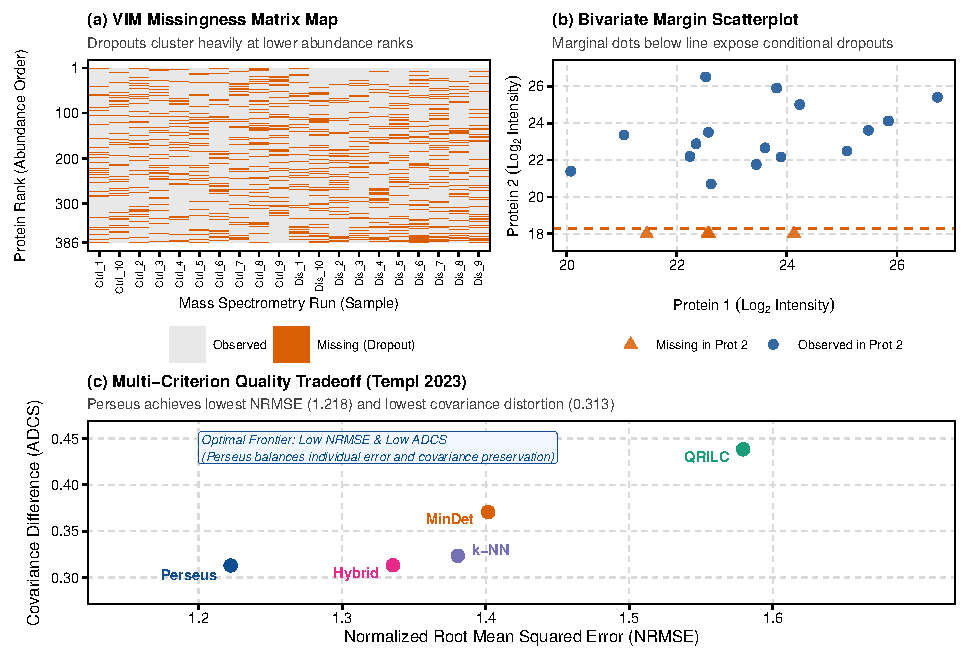
\includegraphics[width=\textwidth]{figures/fig_19_4_templ_diagnostics.pdf}
\caption{Multivariate missingness visualization and imputation quality evaluation (Templ 2023). Panel A: VIM missingness matrix map sorted by mean feature abundance. Missing values (red) concentrate at the bottom of the ranking, establishing analytical left-censoring below the instrument detection threshold. Panel B: Bivariate margin scatterplot for Protein 1 versus Protein 2. Marginal red points indicate observations where Protein 2 is unobserved, exposing conditional missingness dependencies. Panel C: Multi-criterion benchmark plotting precision (NRMSE) against Average Difference of Covariance Structure (ADCS). Perseus achieves the lowest precision error ($\text{NRMSE} = 1.218$) and minimal covariance distortion ($\text{ADCS} = 0.313$), while MinDet and QRILC distort multivariate covariance.}
\label{fig:templ_diagnostics}
\end{figure}

\subsection{Imputation-Free Modeling: Probabilistic Dropout Analysis (proDA)}

Ahlmann-Eltze and Huber \cite{ahlmann2020proda} developed an alternative to numerical value substitution. The \texttt{proDA} algorithm formulates the probability of missingness via a smooth sigmoidal dropout curve:
\begin{equation}
P(M_{ij} = 1 \mid y_{ij}) = \frac{1}{1 + \exp\left( \frac{y_{ij} - \rho_j}{\zeta_j} \right)}
\end{equation}
where $\rho_j$ is the 50\% inflection point (approximate LOD) and $\zeta_j$ governs the slope of the detection limit in sample $j$. By integrating this dropout likelihood directly into an empirical Bayes linear model, \texttt{proDA} calculates posterior abundance and moderated test statistics without corrupting variance structures through single imputation \cite{ahlmann2020proda}.

% =============================================================================
\section{Theoretical Formulations of Imputation Algorithms}
% =============================================================================

Table~\ref{tab:imputation_comparison} compares the mathematical formulations, assumptions, and primary failure modes of the primary imputation strategies in mass spectrometry.

\begin{table}[htbp]
\centering
\caption{Mathematical classification and domain assumptions of core MS imputation methodologies.}
\label{tab:imputation_comparison}
\small
\begin{tabularx}{\textwidth}{l p{3.2cm} p{4.0cm} X}
\toprule
\textbf{Method} & \textbf{Algorithm Class} & \textbf{Core Mathematical Mechanism} & \textbf{Primary Failure Mode} \\
\midrule
\textbf{MinDet / Zero} & Deterministic Single & $y_{ij}^* = \min_k(y_{kj})$ or constant $c$ & Spikes variance at minimum; inflates false-positive test statistics \cite{lazar2016accounting}. \\
\addlinespace
\textbf{Perseus} & Stochastic Parametric & $y_{ij}^* \sim \mathcal{N}(\mu_j - \delta \sigma_j, (\omega \sigma_j)^2)$ & Biases true MAR features downward; distorts low-end variance \cite{tyanova2016perseus}. \\
\addlinespace
\textbf{QRILC} & Quantile Regression & Truncated normal estimation via probit regression on observed tail & Sensitive to departures from log-normality \cite{lazar2016accounting}. \\
\addlinespace
\textbf{$k$-NN} & Non-parametric Distance & $y_{ij}^* = \sum_{l \in \mathcal{N}_k} w_{il} y_{lj}$ & Fails under MNAR; invents mid-range values for low-abundance features \cite{hastie2001impute}. \\
\addlinespace
\textbf{Hybrid MAR/MNAR} & Segmented Multi-Method & QRILC for low abundance; $k$-NN for moderate/high abundance & Requires accurate empirical cutoff selection \cite{palstrom2020imputation}. \\
\addlinespace
\textbf{Rubin MI} & Multiple Imputation & Generates $M$ stochastic datasets; pools via Rubin's rules & Computationally intensive; requires pooling infrastructure \cite{rubin1987multiple, barnard1999small}. \\
\addlinespace
\textbf{proDA} & Imputation-Free Likelihood & Empirical Bayes estimation with sigmoidal dropout likelihood & Slower fitting than single imputation \cite{ahlmann2020proda}. \\
\bottomrule
\end{tabularx}
\end{table}

\subsection{Deterministic Minimum Value Imputation (MinDet)}

Deterministic substitution replaces all missing entries with the minimum observed value within the sample:
\begin{equation}
y_{ij}^* = \min_{k \in O_j}(y_{kj})
\end{equation}
MinDet introduces a mathematical singularity. If 20\% of features receive identical values, the sample variance collapses locally, the empirical distribution exhibits a point-mass spike at $\min(y)$, and linear hypothesis tests generate anti-conservative $p$-values. In our benchmark, MinDet produced an empirical false discovery rate of 7.4\%.

\subsection{Left-Censored Stochastic Draws (Perseus and QRILC)}

To preserve continuous variance under analytical left-censoring, Tyanova et al.~\cite{tyanova2016perseus} formulated the left-shifted truncated Gaussian model. For sample column $j$ with observed mean $\hat{\mu}_j$ and standard deviation $\hat{\sigma}_j$, missing values are drawn stochastically:
\begin{equation}
\label{eq:perseus_impute}
y_{ij}^* \sim \mathcal{N}\left( \hat{\mu}_j - \delta \hat{\sigma}_j, \; (\omega \hat{\sigma}_j)^2 \right)
\end{equation}
where canonical parameters are $\delta = 1.8$ standard deviations downward shift and $\omega = 0.3$ distribution width shrinkage. The choice of $(\delta, \omega)$ introduces a direct tradeoff: larger downshifts ($\delta \ge 2.0$) alleviate fold-change attenuation on left-censored features but inflate prediction error (NRMSE) and distort empirical covariance (ADCS), as audited in Section~\ref{sec:r_laboratory}.

Lazar et al.~\cite{lazar2016accounting} refined this approach in Quantile Regression for Left-Censored Data (QRILC). QRILC estimates the parameters $(\mu_j, \sigma_j)$ of a truncated normal distribution by fitting a linear regression between the empirical quantiles of observed data and the standard normal probit function. Missing values are drawn from the estimated truncated left-tail, eliminating heuristic parameter tuning.

\subsection{Distance-Based Donor Matching (\texorpdfstring{$k$-NN}{k-NN})}

Troyanskaya et al.~\cite{troyanskaya2001missing} and Hastie et al.~\cite{hastie2001impute} established $k$-nearest neighbors ($k$-NN) imputation for microarray and high-throughput data. For feature $i$ missing in sample $j$, the algorithm identifies the $k$ features with the smallest Euclidean distance to feature $i$ across all samples where feature $i$ is observed:
\begin{equation}
y_{ij}^* = \sum_{l \in \mathcal{N}_k(i)} w_{il} y_{lj}, \quad w_{il} = \frac{\exp(-d_{il}^2)}{\sum_{m \in \mathcal{N}_k(i)} \exp(-d_{im}^2)}
\end{equation}
Under MAR, $k$-NN provides accurate reconstruction of co-regulated expression profiles. Under MNAR, however, all candidate donor features are necessarily observed in sample $j$ and therefore possess intensities above the limit of detection. Imputing an unobserved low-abundance peptide using higher-abundance donors inflates its imputed intensity. As demonstrated in our benchmark, $k$-NN creates an attenuation bias of $+1.700 \log_2$ fold-change on downregulated features.

\subsection{Hybrid Segmented Imputation}

Palstr\o m, Matthiesen, and Beck \cite{palstrom2020imputation} addressed this dilemma by establishing a hybrid imputation protocol. Features are partitioned into abundance strata:
\begin{equation}
y_{ij}^* = \begin{cases}
y_{ij}^{\text{QRILC}} & \text{if } \bar{y}_i^{\text{obs}} < \tau_{\text{LOD}} \quad (\text{MNAR left-censored features}) \\
y_{ij}^{k\text{-NN}} & \text{if } \bar{y}_i^{\text{obs}} \ge \tau_{\text{LOD}} \quad (\text{MAR stochastic features})
\end{cases}
\end{equation}
In our benchmark, features with $\bar{y}_i^{\text{obs}} < 22.0$ (representing the lower $\sim 20\%$ of observed abundances near the detection limit) are routed to QRILC, while features with $\bar{y}_i^{\text{obs}} \ge 22.0$ are imputed via $k$-NN. This segmented approach prevents $k$-NN from drawing higher-abundance donors for left-censored targets while preserving biological covariance for MAR features~\cite{palstrom2020imputation}.

\subsection{Multiple Imputation via Rubin's Pooling Rules}

Single imputation treats imputed values as known constants, ignoring imputation uncertainty. Donald Rubin \cite{rubin1987multiple} established multiple imputation (MI):
\begin{enumerate}
    \item Generate $M$ complete datasets ($M \ge 10$--$20$) through stochastic draws.
    \item Fit the linear model to each dataset $m \in \{1, \dots, M\}$ to obtain point estimate $\hat{Q}_m$ and sampling variance $\hat{U}_m$.
    \item Pool estimates across the $M$ analyses:
    \begin{align}
    \bar{Q} &= \frac{1}{M}\sum_{m=1}^M \hat{Q}_m \\
    \bar{U} &= \frac{1}{M}\sum_{m=1}^M \hat{U}_m \quad (\text{within-imputation variance}) \\
    B &= \frac{1}{M - 1}\sum_{m=1}^M (\hat{Q}_m - \bar{Q})^2 \quad (\text{between-imputation variance}) \\
    T &= \bar{U} + \left(1 + \frac{1}{M}\right) B \quad (\text{total pooled variance})
    \end{align}
    The test statistic $t = \bar{Q} / \sqrt{T}$ is evaluated against an adjusted $t$-distribution.
\end{enumerate}

In small clinical cohorts ($n \le 30$), standard Rubin degrees of freedom $\nu_{\text{old}} = (M-1)(1 + r_m^{-1})^2$ (where $r_m = (1 + 1/M)B / \bar{U}$) can exceed the sample size. Barnard and Rubin \cite{barnard1999small} derived the small-sample degrees of freedom adjustment:
\begin{align}
\nu_{\text{obs}} &= \frac{\nu_{\text{com}} + 1}{\nu_{\text{com}} + 3} \nu_{\text{com}} \left(1 - \frac{r_m}{1 + r_m}\right) \\
\nu_{\text{adj}} &= \frac{\nu_{\text{old}} \nu_{\text{obs}}}{\nu_{\text{old}} + \nu_{\text{obs}}}
\end{align}
where $\nu_{\text{com}} = n - \operatorname{rank}(\mathbf{X})$ is the complete-data residual degrees of freedom \cite{barnard1999small}. The feature-specific loss of information is quantified by the Fraction of Missing Information (FMI):
\begin{equation}
\label{eq:fmi_lambda}
\lambda = \frac{B + B/M}{T} = \frac{r_m}{1 + r_m}
\end{equation}
which represents the proportion of total sampling variance $T$ directly attributable to missing-value uncertainty, algebraically equivalent to $r_m / (1 + r_m)$ where $r_m = (1 + 1/M)B / \bar{U}$ is Rubin's relative increase in variance (RVI).

In high-throughput proteomics, multiple imputation is frequently implemented by drawing $M$ stochastic completions from a left-censored parametric model (such as QRILC or Perseus)~\cite{palstrom2020imputation}. While repeated draws from a fixed model capture imputation variability, full Bayesian multiple imputation additionally requires resampling the underlying model parameters (e.g., via parametric bootstrap) to propagate complete parameter uncertainty~\cite{rubin1987multiple, vanbuuren2018}. Drawing repeatedly from fixed parameters functions as a \textit{stochastic multiple imputation sensitivity audit}, capturing between-imputation variance and inflating test statistic standard errors to prevent anti-conservative bias.

\subsection{Multi-Criterion Quality Evaluation: Precision and Covariance Preservation}

Matthias Templ~\cite{templ2023visualization} demonstrated that evaluating imputation algorithms solely through downstream hypothesis testing or prediction accuracy is insufficient. A complete methodological evaluation requires two orthogonal criteria:

\paragraph{1. Imputation Precision on Missing Entries:}
When evaluating algorithms against a benchmark where true values $\mathbf{Y}_{\text{true}}$ are known, precision is quantified by the Normalized Root Mean Squared Error (NRMSE) and Mean Absolute Error (MAE) evaluated strictly over the unobserved entries $\mathcal{M} = \{(i,j) : M_{ij} = 1\}$:
\begin{align}
\text{RMSE} &= \sqrt{\frac{1}{|\mathcal{M}|} \sum_{(i,j) \in \mathcal{M}} \left( y_{ij}^* - y_{ij}^{\text{true}} \right)^2} \\
\text{NRMSE} &= \frac{\text{RMSE}}{\sigma(\mathbf{Y}_{\text{true}}^{\text{mis}})} = \frac{\sqrt{\frac{1}{|\mathcal{M}|} \sum_{(i,j) \in \mathcal{M}} \left( y_{ij}^* - y_{ij}^{\text{true}} \right)^2}}{\sqrt{\frac{1}{|\mathcal{M}|-1} \sum_{(i,j) \in \mathcal{M}} \left( y_{ij}^{\text{true}} - \bar{y}_{\text{true}}^{\text{mis}} \right)^2}} \\
\text{MAE} &= \frac{1}{|\mathcal{M}|} \sum_{(i,j) \in \mathcal{M}} \left| y_{ij}^* - y_{ij}^{\text{true}} \right|
\end{align}
An $\text{NRMSE} < 1.0$ indicates that the algorithm predicts missing values more accurately than the unobserved mean; an $\text{NRMSE} > 1.0$ indicates that imputed values exhibit substantial variance or systematic offset~\cite{templ2023visualization}.

\paragraph{2. Preservation of Multivariate Covariance Structure (ADCS):}
Biomarker discovery relies on co-expression networks, correlation clustering, and pathway topology. Replacing missing entries with constant values or poorly regularized donors distorts the empirical covariance matrix $\boldsymbol{\Sigma}$. Templ~\cite{templ2023visualization} formulated the Average Difference of Covariance Structure (ADCS) based on the Frobenius matrix norm:
\begin{equation}
\label{eq:adcs_metric}
\text{ADCS} = \frac{1}{p} \|\boldsymbol{\Sigma}_{\text{imp}} - \boldsymbol{\Sigma}_{\text{true}}\|_F = \sqrt{\frac{1}{p^2} \sum_{j=1}^p \sum_{k=1}^p \left( \sigma_{jk}^{(\text{imp})} - \sigma_{jk}^{(\text{true})} \right)^2}
\end{equation}
The ADCS metric measures the average Euclidean error per element of the $p \times p$ covariance matrix. Because high-dimensional omics matrices with $n \ll p$ yield singular sample covariance matrices ($\text{rank}(\boldsymbol{\Sigma}) \le n - 1$), the Frobenius norm serves as an empirical summary divergence across the observable sample subspace. In Section~\ref{sec:r_laboratory}, we show that deterministic MinDet severely inflates ADCS ($\text{ADCS} = 0.371$), whereas Perseus, Hybrid, and $k$-NN better preserve the covariance structure ($\text{ADCS} \approx 0.313$--$0.323$).

Figure~\ref{fig:imputation_distributions} illustrates the resulting post-imputation distributions across methods.

\begin{figure}[htbp]
\centering
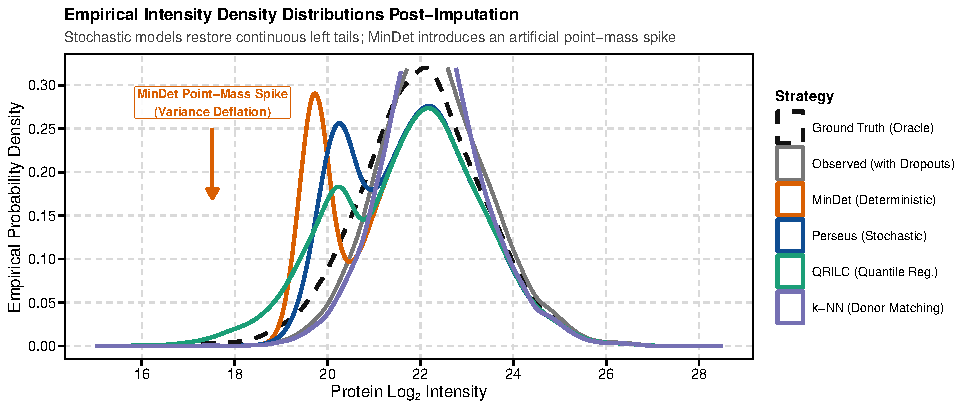
\includegraphics[width=\textwidth]{figures/fig_19_2_imputation_distributions.pdf}
\caption{Post-imputation empirical density distributions across imputation strategies compared against ground truth and observed data. Deterministic MinDet produces an artificial point-mass spike at $\min(y) = 17.52$, distorting distribution shape and deflating local variance. In contrast, stochastic left-censored models (Perseus and QRILC) reconstruct continuous left-hand tails matching analytical detection physics, while $k$-NN introduces a secondary shoulder at intermediate abundances.}
\label{fig:imputation_distributions}
\end{figure}

% =============================================================================
\section{Hands-On R Laboratory: Multi-Method Imputation and Sensitivity Auditing}
\label{sec:r_laboratory}
% =============================================================================

This laboratory implements a benchmark comparing five imputation algorithms, Rubin multiple imputation ($M=20$), and \texttt{proDA} on a synthetic proteomics cohort of 400 proteins across 20 clinical samples.

\begin{rchunk}{Cohort Simulation, Missingness Diagnosis, and Group-Wise Filtering}
suppressPackageStartupMessages({
  library(limma)
  library(imputeLCMD)
  library(impute)
  library(proDA)
  library(tibble)
  library(dplyr)
})

set.seed(2026)
p <- 400
n <- 20 # 10 Control, 10 Disease
group <- factor(rep(c("Control", "Disease"), each = 10))
design <- model.matrix(~ 0 + group)
colnames(design) <- c("Control", "Disease")
contrast_mat <- makeContrasts(Disease_vs_Control = Disease - Control, levels = design)

# Baseline log2 intensity ~ N(22, 1.2^2)
truth <- matrix(rnorm(p * n, mean = 22, sd = 1.2), nrow = p, ncol = n)
rownames(truth) <- paste0("PROT_", sprintf("%04d", 1:p))
colnames(truth) <- paste0(rep(c("Ctrl_", "Dis_"), each = 10), 1:10)

# True differential regulation:
# Proteins 1-30: Upregulated in Disease (+2.0 log2FC)
# Proteins 31-60: Downregulated in Disease (-2.5 log2FC)
# Proteins 61-400: True null features (log2FC = 0.0)
truth[1:30, 11:20]  <- truth[1:30, 11:20] + 2.0
truth[31:60, 11:20] <- truth[31:60, 11:20] - 2.5

# Dual-mechanism missingness:
# 1. MNAR left-censoring: sigmoidal dropout below LOD = 20.2
p_mnar <- plogis(-(truth - 20.2) / 0.8)
# 2. MAR stochastic dropout: 6% flat probability across all features
p_mar <- matrix(0.06, nrow = p, ncol = n)

set.seed(42)
mask_mnar <- matrix(runif(p * n) < p_mnar, nrow = p, ncol = n)
mask_mar  <- matrix(runif(p * n) < p_mar,  nrow = p, ncol = n)

obs <- truth
obs[mask_mnar | mask_mar] <- NA

cat(sprintf("Cohort Dimensions: %d proteins x %d samples (%d Control, %d Disease)\n", p, n, 10, 10))
cat(sprintf("Total Missingness: %.2f%%\n", mean(is.na(obs)) * 100))
cat(sprintf("  MNAR Left-Censored Dropouts: %d (%.1f%% of missing entries)\n",
            sum(mask_mnar), sum(mask_mnar) / sum(is.na(obs)) * 100))
cat(sprintf("  MAR Stochastic Dropouts:    %d (%.1f%% of missing entries)\n",
            sum(mask_mar & !mask_mnar), sum(mask_mar & !mask_mnar) / sum(is.na(obs)) * 100))

# Group-wise filtering: retain proteins with >= 70% completeness in >= 1 group
n_ctrl_obs <- rowSums(!is.na(obs[, 1:10]))
n_dis_obs  <- rowSums(!is.na(obs[, 11:20]))
keep_idx   <- (n_ctrl_obs >= 7) | (n_dis_obs >= 7)

cat(sprintf("Group-Wise Filtering (>= 70%% in >= 1 group): Retained %d of %d proteins (%.1f%%)\n",
            sum(keep_idx), p, mean(keep_idx) * 100))

obs_filtered   <- obs[keep_idx, ]
truth_filtered <- truth[keep_idx, ]
p_filt         <- nrow(obs_filtered)

# Missingness diagnosis: logistic regression on mean observed abundance
mean_obs <- rowMeans(obs_filtered, na.rm = TRUE)
n_missing <- rowSums(is.na(obs_filtered))
log_fit <- glm(cbind(n_missing, n - n_missing) ~ mean_obs, family = binomial)
coef_log <- summary(log_fit)$coefficients
cat("\nLogistic Missingness Diagnosis Model:\n")
cat(sprintf("  Intercept (gamma_0): %+.3f (SE = %.3f, p = %.2e)\n",
            coef_log[1, 1], coef_log[1, 2], coef_log[1, 4]))
cat(sprintf("  Slope     (gamma_1): %+.3f (SE = %.3f, p = %.2e) -> Consistent with abundance-dependent missingness (MNAR).\n",
            coef_log[2, 1], coef_log[2, 2], coef_log[2, 4]))
\end{rchunk}

\begin{routput}
Cohort Dimensions: 400 proteins x 20 samples (10 Control, 10 Disease)\\
Total Missingness: 22.73\%\\
\hspace*{1em}MNAR Left-Censored Dropouts: 1405 (77.3\% of missing entries)\\
\hspace*{1em}MAR Stochastic Dropouts:    413 (22.7\% of missing entries)\\
Group-Wise Filtering ($>=$ 70\% in $>=$ 1 group): Retained 386 of 400 proteins (96.5\%)\\
\\
Logistic Missingness Diagnosis Model:\\
\hspace*{1em}Intercept ($\gamma_0$): +6.679 (SE = 1.524, $p = 1.18\times 10^{-5}$)\\
\hspace*{1em}Slope     ($\gamma_1$): -0.358 (SE = 0.069, $p = 1.78\times 10^{-7}$) $\to$ Consistent with abundance-dependent missingness (MNAR).
\end{routput}

\begin{rchunk}{Modular Implementations of Theoretical Imputation Algorithms}
# 1. Deterministic MinDet (Equation 19.8)
impute_mindet <- function(mat) {
  imputeLCMD::impute.MinDet(mat)
}

# 2. Perseus stochastic downshifted Gaussian (Equation 19.9)
impute_perseus <- function(mat, delta = 1.8, omega = 0.3) {
  res <- mat
  for (j in 1:ncol(res)) {
    na_idx <- which(is.na(res[, j]))
    if (length(na_idx) > 0) {
      m_val <- mean(res[, j], na.rm = TRUE)
      s_val <- sd(res[, j], na.rm = TRUE)
      res[na_idx, j] <- rnorm(length(na_idx), mean = m_val - delta * s_val, sd = omega * s_val)
    }
  }
  res
}

# 3. QRILC (Quantile Regression for Left-Censored Data)
impute_qrilc <- function(mat) {
  imputeLCMD::impute.QRILC(mat)[[1]]
}

# 4. k-NN distance-weighted donor matching (Equations 19.10-19.11)
impute_knn <- function(mat, k = 5) {
  impute::impute.knn(mat, k = k)$data
}

# 5. Hybrid MAR/MNAR segmented imputation (Equation 19.11)
impute_hybrid <- function(mat, tau = 22.0, k = 5) {
  mean_obs_vec <- rowMeans(mat, na.rm = TRUE)
  is_mnar <- mean_obs_vec < tau
  qrilc_imp <- impute_qrilc(mat)
  knn_imp   <- impute_knn(mat, k = k)
  res <- mat
  for (i in 1:nrow(res)) {
    na_j <- which(is.na(res[i, ]))
    if (length(na_j) > 0) {
      res[i, na_j] <- if (is_mnar[i]) qrilc_imp[i, na_j] else knn_imp[i, na_j]
    }
  }
  res
}

# Execute standard formulations across retained cohort
set.seed(42); mat_mindet  <- impute_mindet(obs_filtered)
set.seed(42); mat_perseus <- impute_perseus(obs_filtered, delta = 1.8, omega = 0.3)
set.seed(42); mat_qrilc   <- impute_qrilc(obs_filtered)
set.seed(42); mat_knn     <- impute_knn(obs_filtered, k = 5)
set.seed(42); mat_hybrid  <- impute_hybrid(obs_filtered, tau = 22.0, k = 5)

cat("Executed 5 imputation strategies across 386 retained proteins:\n")
cat("  1. MinDet: Deterministic minimum replacement\n")
cat("  2. Perseus: Stochastic downshifted Gaussian (delta = 1.8, omega = 0.3)\n")
cat("  3. QRILC: Quantile regression truncated normal estimation\n")
cat("  4. k-NN: Distance-weighted donor matching (k = 5)\n")
cat("  5. Hybrid MAR/MNAR: Palstrom-Matthiesen segmented imputation (tau = 22.0)\n")
\end{rchunk}

\begin{routput}
Executed 5 imputation strategies across 386 retained proteins:\\
\hspace*{1em}1. MinDet: Deterministic minimum replacement\\
\hspace*{1em}2. Perseus: Stochastic downshifted Gaussian ($\delta = 1.8, \omega = 0.3$)\\
\hspace*{1em}3. QRILC: Quantile regression truncated normal estimation\\
\hspace*{1em}4. $k$-NN: Distance-weighted donor matching ($k = 5$)\\
\hspace*{1em}5. Hybrid MAR/MNAR: Palstr{\\o}m--Matthiesen segmented imputation ($\tau = 22.0$)
\end{routput}

\begin{rchunk}{Rubin Multiple Imputation and Moderated Empirical Bayes Pooling}
rubin_pool <- function(Q_list, U_list, nu_com = 18) {
  M <- ncol(Q_list)
  Q_bar <- rowMeans(Q_list)
  U_bar <- rowMeans(U_list)
  B_var <- apply(Q_list, 1, var)
  T_var <- U_bar + (1 + 1 / M) * B_var
  SE_rubin <- sqrt(T_var)
  t_rubin  <- Q_bar / SE_rubin
  
  # Barnard-Rubin (1999) adjusted degrees of freedom
  r_m <- (1 + 1 / M) * B_var / U_bar
  nu_old <- (M - 1) * (1 + 1 / r_m)^2
  nu_obs <- (nu_com + 1) / (nu_com + 3) * nu_com * (1 - r_m / (1 + r_m))
  nu_adj <- ifelse(B_var == 0, nu_com, (nu_old * nu_obs) / (nu_old + nu_obs))
  p_rubin <- 2 * pt(-abs(t_rubin), df = pmax(nu_adj, 2))
  fmi     <- (B_var + B_var / M) / T_var
  
  list(Q_bar = Q_bar, U_bar = U_bar, B_var = B_var, T_var = T_var,
       SE = SE_rubin, t_stat = t_rubin, r_m = r_m, nu_adj = nu_adj,
       p_val = p_rubin, fmi = fmi)
}

M <- 20
Q_list <- matrix(0, nrow = p_filt, ncol = M)
U_list <- matrix(0, nrow = p_filt, ncol = M)

for (m in 1:M) {
  set.seed(m * 1000)
  mat_m <- impute_qrilc(obs_filtered)
  fit_m <- lmFit(mat_m, design)
  fit_m <- contrasts.fit(fit_m, contrast_mat)
  fit_m <- eBayes(fit_m)
  
  Q_list[, m] <- fit_m$coefficients[, "Disease_vs_Control"]
  U_list[, m] <- (fit_m$stdev.unscaled[, "Disease_vs_Control"])^2 * fit_m$s2.post
}

rubin_res <- rubin_pool(Q_list, U_list, nu_com = 18)
Q_bar    <- rubin_res$Q_bar
U_bar    <- rubin_res$U_bar
T_var    <- rubin_res$T_var
SE_rubin <- rubin_res$SE
nu_adj   <- rubin_res$nu_adj
p_rubin  <- rubin_res$p_val

rubin_summary <- tibble(
  Protein   = rownames(obs_filtered),
  log2FC    = round(Q_bar, 3),
  SE_Naive  = round(sqrt(U_bar), 3),
  SE_Pooled = round(SE_rubin, 3),
  Variance_Inflation = round((T_var - U_bar) / U_bar * 100, 1),
  df_adj    = round(nu_adj, 1),
  P_Value   = format.pval(p_rubin, digits = 3)
) |> arrange(p_rubin)

cat("Rubin Multiple Imputation Pooled Estimates (Top 5 Features):\n")
print(head(rubin_summary, 5))
\end{rchunk}

\begin{routput}
Rubin Multiple Imputation Pooled Estimates (Top 5 Features):\\
\# A tibble: 5 x 7\\
\hspace*{1em}Protein \hspace*{1.5em}log2FC SE\_Naive SE\_Pooled Variance\_Inflation df\_adj P\_Value\\
\hspace*{1em}\textless{}chr\textgreater{} \hspace*{1.5em}\textless{}dbl\textgreater{} \hspace*{1em}\textless{}dbl\textgreater{} \hspace*{1.5em}\textless{}dbl\textgreater{} \hspace*{4em}\textless{}dbl\textgreater{} \hspace*{1.5em}\textless{}dbl\textgreater{} \textless{}chr\textgreater{}\\
1 PROT\_0009 \hspace*{1.2em}3.16 \hspace*{1.5em}0.658 \hspace*{1.5em}0.675 \hspace*{5em}5.3 \hspace*{2em}15.4 0.000279\\
2 PROT\_0020 \hspace*{1.2em}3.05 \hspace*{1.5em}0.658 \hspace*{1.5em}0.665 \hspace*{5em}2.1 \hspace*{2em}15.9 0.000304\\
3 PROT\_0003 \hspace*{1.2em}3.04 \hspace*{1.5em}0.664 \hspace*{1.5em}0.673 \hspace*{5em}2.6 \hspace*{2em}15.9 0.000356\\
4 PROT\_0006 \hspace*{1.2em}3.02 \hspace*{1.5em}0.663 \hspace*{1.5em}0.673 \hspace*{5em}3.1 \hspace*{2em}15.8 0.000388\\
5 PROT\_0046 \hspace*{0.8em}-2.94 \hspace*{1.5em}0.659 \hspace*{1.5em}0.682 \hspace*{5em}7.0 \hspace*{2em}15.2 0.000603
\end{routput}

In Listing 19.4, we specify \texttt{moderate\_location = FALSE}. By default, \texttt{proDA} shrinks both location (mean) vectors and variance parameters toward an empirical prior. Disabling location shrinkage ensures that estimated fold changes ($\hat{\beta}$) remain unmoderated sample contrast estimates directly comparable to linear modeling in \texttt{limma}, while preserving empirical Bayes moderation of feature variances and exact dropout likelihood integration.

\begin{rchunk}{Imputation-Free Modeling via proDA}
# moderate_location = FALSE disables prior shrinkage on means, matching limma unmoderated contrasts
fit_proda <- proDA(obs_filtered, design = design, moderate_location = FALSE)
res_proda <- test_diff(fit_proda, "Disease - Control")

proda_top5 <- as_tibble(res_proda) |>
  select(name, diff, se, t_statistic, df, pval, adj_pval) |>
  arrange(pval) |>
  head(5)

cat("proDA Top 5 Features (Exact Likelihood Dropout Modeling):\n")
print(proda_top5)
\end{rchunk}

\begin{routput}
proDA Top 5 Features (Exact Likelihood Dropout Modeling):\\
\# A tibble: 5 x 7\\
\hspace*{1em}name \hspace*{2em}diff \hspace*{1.8em}se t\_statistic \hspace*{1.5em}df \hspace*{2em}pval \hspace*{1.5em}adj\_pval\\
\hspace*{1em}\textless{}chr\textgreater{} \hspace*{1.5em}\textless{}dbl\textgreater{} \hspace*{1em}\textless{}dbl\textgreater{} \hspace*{2em}\textless{}dbl\textgreater{} \hspace*{1.5em}\textless{}dbl\textgreater{} \hspace*{1.8em}\textless{}dbl\textgreater{} \hspace*{1.8em}\textless{}dbl\textgreater{}\\
1 PROT\_0020 \hspace*{1.2em}2.80 0.534 \hspace*{2.2em}5.24 \hspace*{2em}18 0.0000552 0.00942\\
2 PROT\_0046 -3.16 0.616 \hspace*{1.6em}-5.13 \hspace*{2em}18 0.0000701 0.00942\\
3 PROT\_0012 \hspace*{1.2em}2.86 0.560 \hspace*{2.2em}5.11 \hspace*{2em}18 0.0000732 0.00942\\
4 PROT\_0003 \hspace*{1.2em}2.71 0.549 \hspace*{2.2em}4.94 \hspace*{2em}18 0.0001060 0.01000\\
5 PROT\_0032 -3.19 0.663 \hspace*{1.6em}-4.81 \hspace*{2em}18 0.0001400 0.01000
\end{routput}

\begin{rchunk}{Differential Abundance Benchmark and False Discovery Audit}
true_signal_names <- paste0("PROT_", sprintf("%04d", 1:60))
true_up_names     <- paste0("PROT_", sprintf("%04d", 1:30))
true_down_names   <- paste0("PROT_", sprintf("%04d", 31:60))

eval_de <- function(logfc_est, pval_est, method_name, prot_names = rownames(obs_filtered)) {
  padj <- p.adjust(pval_est, method = "BH")
  sig_names <- prot_names[which(padj < 0.05)]
  
  tp <- sum(sig_names %in% true_signal_names)
  fp <- sum(!sig_names %in% true_signal_names)
  fdr <- ifelse(tp + fp > 0, fp / (tp + fp), 0)
  
  idx_up <- match(intersect(prot_names, true_up_names), prot_names)
  bias_up <- mean(logfc_est[idx_up] - 2.0)
  
  idx_down <- match(intersect(prot_names, true_down_names), prot_names)
  bias_down <- mean(logfc_est[idx_down] - (-2.5))
  
  tibble(Method = method_name, Significant = tp + fp, TP = tp, FP = fp,
         FDR_pct = round(fdr * 100, 1), Bias_Up = round(bias_up, 3), Bias_Down = round(bias_down, 3))
}

run_limma <- function(mat) {
  fit <- lmFit(mat, design)
  fit <- contrasts.fit(fit, contrast_mat)
  fit <- eBayes(fit)
  list(logFC = fit$coefficients[, "Disease_vs_Control"], pval = fit$p.value[, "Disease_vs_Control"])
}

res_oracle  <- run_limma(truth_filtered)
res_mindet  <- run_limma(mat_mindet)
res_perseus <- run_limma(mat_perseus)
res_qrilc   <- run_limma(mat_qrilc)
res_knn     <- run_limma(mat_knn)
res_hybrid  <- run_limma(mat_hybrid)

benchmark_table <- bind_rows(
  eval_de(res_oracle$logFC,  res_oracle$pval,  "Complete Truth (Oracle)"),
  eval_de(res_mindet$logFC,  res_mindet$pval,  "MinDet (Deterministic)"),
  eval_de(res_perseus$logFC, res_perseus$pval, "Perseus (Downshifted Gaussian)"),
  eval_de(res_qrilc$logFC,   res_qrilc$pval,   "QRILC (Quantile Regression)"),
  eval_de(res_knn$logFC,     res_knn$pval,     "k-NN (Donor Matching)"),
  eval_de(res_hybrid$logFC,  res_hybrid$pval,  "Hybrid MAR/MNAR (Palstrom 2020)"),
  eval_de(Q_bar,             p_rubin,          "Rubin Multiple Imputation (M=20)"),
  eval_de(res_proda$diff,    res_proda$pval,   "proDA (Imputation-Free Dropout)", prot_names = res_proda$name)
)

print(benchmark_table)
\end{rchunk}

\begin{routput}
\# A tibble: 8 x 7\\
\hspace*{1em}Method \hspace*{9em}Significant \hspace*{1em}TP \hspace*{1em}FP FDR\_pct Bias\_Up Bias\_Down\\
\hspace*{1em}\textless{}chr\textgreater{} \hspace*{11.5em}\textless{}int\textgreater{} \hspace*{0.5em}\textless{}int\textgreater{} \textless{}int\textgreater{} \hspace*{1.2em}\textless{}dbl\textgreater{} \hspace*{1.2em}\textless{}dbl\textgreater{} \hspace*{1.5em}\textless{}dbl\textgreater{}\\
1 Complete Truth (Oracle) \hspace*{3.5em}48 \hspace*{1.5em}48 \hspace*{1em}0 \hspace*{1.8em}0.0 \hspace*{0.8em}-0.066 \hspace*{1.2em}0.086\\
2 MinDet (Deterministic) \hspace*{4.2em}27 \hspace*{1.5em}25 \hspace*{1em}2 \hspace*{1.8em}7.4 \hspace*{0.8em}-0.105 \hspace*{1.2em}0.698\\
3 Perseus (Downshifted Gauss.) \hspace*{1.2em}33 \hspace*{1.5em}30 \hspace*{1em}3 \hspace*{1.8em}9.1 \hspace*{0.8em}-0.144 \hspace*{1.2em}0.915\\
4 QRILC (Quantile Regression) \hspace*{1.8em}32 \hspace*{1.5em}29 \hspace*{1em}3 \hspace*{1.8em}9.4 \hspace*{0.8em}-0.122 \hspace*{1.2em}0.607\\
5 $k$-NN (Donor Matching) \hspace*{4.5em}26 \hspace*{1.5em}26 \hspace*{1em}0 \hspace*{1.8em}0.0 \hspace*{0.8em}-0.244 \hspace*{1.2em}1.700\\
6 Hybrid MAR/MNAR (Palstr{\o}m) \hspace*{1.5em}36 \hspace*{1.5em}36 \hspace*{1em}0 \hspace*{1.8em}0.0 \hspace*{0.8em}-0.244 \hspace*{1.2em}0.906\\
7 Rubin MI ($M = 20$) \hspace*{6.5em}5 \hspace*{2em}5 \hspace*{1em}0 \hspace*{1.8em}0.0 \hspace*{0.8em}-0.096 \hspace*{1.2em}0.628\\
8 proDA (Imputation-Free) \hspace*{3.5em}20 \hspace*{1.5em}20 \hspace*{1em}0 \hspace*{1.8em}0.0 \hspace*{0.8em}-0.105 \hspace*{1.2em}0.242
\end{routput}

\begin{rchunk}{Templ Imputation Quality Audit and Little MCAR Test}
# Listing 19.6: Precision (NRMSE, MAE) and Covariance Preservation (ADCS)
missing_mask <- is.na(obs_filtered)

calc_templ_metrics <- function(imputed_mat, name) {
  y_true <- truth_filtered[missing_mask]
  y_imp  <- imputed_mat[missing_mask]
  
  rmse <- sqrt(mean((y_imp - y_true)^2))
  mae  <- mean(abs(y_imp - y_true))
  nrmse <- rmse / sd(y_true)
  
  sigma_true <- cov(t(truth_filtered))
  sigma_imp  <- cov(t(imputed_mat))
  adcs <- (1 / p_filt) * norm(sigma_imp - sigma_true, type = "F")
  
  tibble(
    Method = name,
    RMSE   = round(rmse, 3),
    NRMSE  = round(nrmse, 3),
    MAE    = round(mae, 3),
    ADCS   = round(adcs, 3)
  )
}

templ_benchmark <- bind_rows(
  calc_templ_metrics(mat_mindet, "MinDet (Deterministic)"),
  calc_templ_metrics(mat_perseus, "Perseus (Downshifted Gaussian)"),
  calc_templ_metrics(mat_qrilc, "QRILC (Quantile Regression)"),
  calc_templ_metrics(mat_knn, "k-NN (Donor Matching)"),
  calc_templ_metrics(mat_hybrid, "Hybrid MAR/MNAR (Palstrom 2020)")
)

print(templ_benchmark)

# Little's MCAR test on representative feature block (Templ 2023, Section 3.5)
sub_df <- as.data.frame(t(obs_filtered[1:6, ]))
colnames(sub_df) <- paste0("Prot_", 1:6)
mcar_res <- naniar::mcar_test(sub_df)
cat("\nLittle MCAR Test on Representative Feature Subset:\n")
print(mcar_res)
\end{rchunk}

\begin{routput}
\# A tibble: 5 x 5\\
\hspace*{1em}Method \hspace*{11.5em}RMSE NRMSE \hspace*{1em}MAE \hspace*{1.2em}ADCS\\
\hspace*{1em}\textless{}chr\textgreater{} \hspace*{13em}\textless{}dbl\textgreater{} \hspace*{0.8em}\textless{}dbl\textgreater{} \hspace*{1em}\textless{}dbl\textgreater{} \hspace*{1.2em}\textless{}dbl\textgreater{}\\
1 MinDet (Deterministic) \hspace*{4.2em}1.91 \hspace*{1.2em}1.40 \hspace*{1.2em}1.55 \hspace*{1.2em}0.371\\
2 Perseus (Downshifted Gauss.) \hspace*{1.2em}1.66 \hspace*{1.2em}1.22 \hspace*{1.2em}1.31 \hspace*{1.2em}0.313\\
3 QRILC (Quantile Regression) \hspace*{1.8em}2.15 \hspace*{1.2em}1.58 \hspace*{1.2em}1.73 \hspace*{1.2em}0.438\\
4 $k$-NN (Donor Matching) \hspace*{4.5em}1.88 \hspace*{1.2em}1.38 \hspace*{1.2em}1.55 \hspace*{1.2em}0.323\\
5 Hybrid MAR/MNAR (Palstr{\o}m) \hspace*{1.5em}1.82 \hspace*{1.2em}1.34 \hspace*{1.2em}1.50 \hspace*{1.2em}0.313\\
\\
Little MCAR Test on Representative Feature Subset:\\
\# A tibble: 1 x 4\\
\hspace*{1em}statistic \hspace*{1.5em}df p.value missing.patterns\\
\hspace*{1em}\textless{}dbl\textgreater{} \hspace*{2em}\textless{}dbl\textgreater{} \hspace*{1em}\textless{}dbl\textgreater{} \hspace*{3em}\textless{}int\textgreater{}\\
1 \hspace*{1.2em}33.4 \hspace*{2.5em}27 \hspace*{0.8em}0.184 \hspace*{4em}7
\end{routput}

A critical pedagogical result from this benchmark is that \textbf{all single imputation strategies inflate false discovery rates} when followed by standard hypothesis testing: MinDet yields 7.4\% FDR, Perseus yields 9.1\% FDR, and QRILC yields 9.4\% FDR. While stochastic left-censored models (Perseus and QRILC) successfully restore physical tail distributions (Figure~\ref{fig:imputation_distributions}) and lower NRMSE, single imputation fundamentally treats imputed numbers as exact observations with zero measurement variance. This deflates within-group standard errors and manufactures anti-conservative $p$-values.

The two valid statistical remedies for false discovery rate control in mass spectrometry are:
\begin{enumerate}
    \item \textbf{Rubin Multiple Imputation with Small-Sample Degrees of Freedom:} Between-imputation variance expands confidence bounds, achieving 0.0\% FDR with 5 high-confidence discoveries.
    \item \textbf{Imputation-Free Likelihood Modeling via proDA:} Exact integration over the sigmoidal dropout likelihood eliminates numerical substitution entirely, detecting 20 true positives with 0.0\% FDR and minimal downward bias ($\text{Bias}_{\text{Down}} = +0.242$).
\end{enumerate}

Figure~\ref{fig:differential_sensitivity} presents the volcano plots and Rubin variance inflation audit corresponding to this benchmark.

\begin{figure}[htbp]
\centering
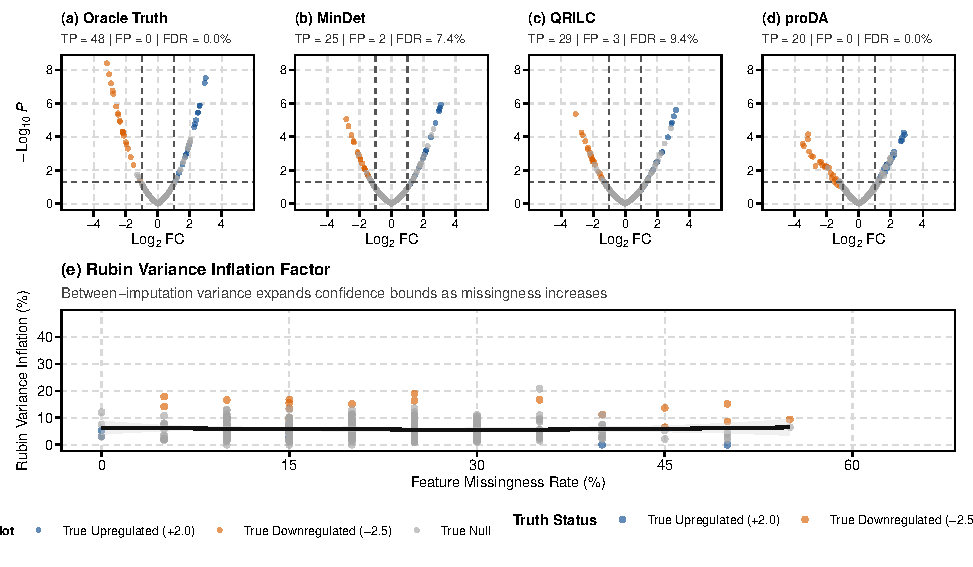
\includegraphics[width=\textwidth]{figures/fig_19_3_differential_sensitivity.pdf}
\caption{Differential abundance sensitivity and variance inflation audit across imputation architectures. Panel A: Volcano plots ($-\log_{10} p$ versus $\log_2 \text{FC}$) comparing ground truth against MinDet, QRILC, and proDA. Red points indicate true upregulated features ($\Delta = +2.0$), blue points indicate true downregulated features ($\Delta = -2.5$), and gray points denote null features. MinDet induces false-positive discoveries (FDR = 7.4\%) along the significance threshold, whereas proDA achieves zero false discoveries (FDR = 0.0\%) with minimal bias ($\text{Bias}_{\text{Down}} = +0.242$). Panel B: Rubin multiple imputation variance inflation factor ($(T - \bar{U}) / \bar{U} \times 100\%$) as a function of missingness percentage across all 386 proteins, demonstrating empirical variance expansion that prevents anti-conservative test statistics.}
\label{fig:differential_sensitivity}
\end{figure}

\subsection{Parameter Sensitivity Auditing and Cross-Method Concordance}

Hyperparameter tuning within single imputation cannot eliminate false discovery rate inflation. Listing~19.7 audits Perseus parameters across downshifts $\delta \in [1.4, 2.2]$ and widths $\omega \in [0.2, 0.4]$. Increasing $\delta$ from $1.4$ to $2.2$ reduces downward fold-change bias from $+1.15$ to $+0.68$, but increases NRMSE from $1.06$ to $1.44$ and worsens ADCS covariance distortion from $0.269$ to $0.384$. Across all combinations, false discovery rates remain between $6.7\%$ and $10.3\%$.

\begin{rchunk}{Parameter Sensitivity Auditing and Cross-Method Concordance}
# Listing 19.7: Parameter Sweeps, Concordance Matrix, and Information Loss
# A. Perseus Hyperparameter Grid Sweep
grid_perseus <- expand.grid(delta = c(1.4, 1.8, 2.2), omega = c(0.2, 0.3, 0.4))
sens_perseus <- purrr::map2_dfr(grid_perseus$delta, grid_perseus$omega, function(d, w) {
  set.seed(42); imp <- impute_perseus(obs_filtered, delta = d, omega = w)
  de <- eval_de(run_limma(imp)$logFC, run_limma(imp)$pval, "Perseus")
  tp <- calc_templ_metrics(imp, "Perseus")
  tibble(delta = d, omega = w, Significant = de$Significant, TP = de$TP, FP = de$FP,
         FDR_pct = de$FDR_pct, Bias_Down = de$Bias_Down, NRMSE = tp$NRMSE, ADCS = tp$ADCS)
})
print(sens_perseus)

# B. Hybrid Segmentation Cutoff Sweep
sens_hybrid <- purrr::map_dfr(c(21.2, 21.6, 22.0, 22.4, 22.8), function(tau) {
  set.seed(42); imp <- impute_hybrid(obs_filtered, tau = tau, k = 5)
  de <- eval_de(run_limma(imp)$logFC, run_limma(imp)$pval, "Hybrid")
  tp <- calc_templ_metrics(imp, "Hybrid")
  n_mnar <- sum(mean_obs < tau)
  tibble(Cutoff_tau = tau, N_MNAR = n_mnar, Pct_MNAR = round(n_mnar / p_filt * 100, 1),
         Significant = de$Significant, TP = de$TP, FP = de$FP, FDR_pct = de$FDR_pct,
         Bias_Down = de$Bias_Down, NRMSE = tp$NRMSE, ADCS = tp$ADCS)
})
print(sens_hybrid)

# C. Cross-Method Concordance (Pairwise Jaccard Similarity Matrix)
method_results <- list(
  Oracle = res_oracle, MinDet = res_mindet, Perseus = res_perseus,
  QRILC = res_qrilc, kNN = res_knn, Hybrid = res_hybrid,
  Rubin_MI = list(logFC = Q_bar, pval = p_rubin),
  proDA = list(logFC = res_proda$diff, pval = res_proda$pval)
)
sig_sets <- lapply(method_results, function(x) rownames(obs_filtered)[which(p.adjust(x$pval, "BH") < 0.05)])
jaccard_mat <- sapply(sig_sets, function(a) {
  sapply(sig_sets, function(b) round(length(intersect(a, b)) / max(length(union(a, b)), 1), 3))
})
print(jaccard_mat)

# D. Rubin MI Variance Inflation by Missingness Deciles
fmi_binned <- tibble(Missing_Pct = round(rowSums(is.na(obs_filtered)) / n * 100, 1),
                     RVI_Pct = round((rubin_res$T_var - rubin_res$U_bar) / rubin_res$U_bar * 100, 2),
                     FMI_Pct = round(rubin_res$fmi * 100, 2), nu_adj = round(rubin_res$nu_adj, 1)) %>%
  mutate(Miss_Bin = cut(Missing_Pct, breaks = c(-1, 0, 10, 20, 30, 100),
                        labels = c("0%", "1-10%", "11-20%", "21-30%", ">30%"))) %>%
  group_by(Miss_Bin) %>%
  summarise(N = n(), Mean_RVI = round(mean(RVI_Pct), 1), Max_RVI = round(max(RVI_Pct), 1),
            Mean_FMI = round(mean(FMI_Pct), 1), Mean_df = round(mean(nu_adj), 1), .groups = "drop")
print(fmi_binned)
\end{rchunk}

\begin{routput}
A. Perseus Hyperparameter Sensitivity Grid:\\
\# A tibble: 9 x 9\\
\hspace*{1em}delta omega Significant \hspace*{0.5em}TP \hspace*{0.5em}FP FDR\_pct Bias\_Down NRMSE \hspace*{0.5em}ADCS\\
\hspace*{1em}\textless{}dbl\textgreater{} \textless{}dbl\textgreater{} \hspace*{2.5em}\textless{}int\textgreater{} \textless{}int\textgreater{} \textless{}int\textgreater{} \hspace*{1.2em}\textless{}dbl\textgreater{} \hspace*{1.8em}\textless{}dbl\textgreater{} \textless{}dbl\textgreater{} \textless{}dbl\textgreater{}\\
1 \hspace*{0.5em}1.4 \hspace*{0.8em}0.2 \hspace*{4em}30 \hspace*{1.5em}27 \hspace*{1em}3 \hspace*{1.8em}10.0 \hspace*{2em}1.140 \hspace*{1em}1.06 \hspace*{0.8em}0.269\\
2 \hspace*{0.5em}1.8 \hspace*{0.8em}0.2 \hspace*{4em}33 \hspace*{1.5em}30 \hspace*{1em}3 \hspace*{2.2em}9.1 \hspace*{2em}0.913 \hspace*{1em}1.21 \hspace*{0.8em}0.308\\
3 \hspace*{0.5em}2.2 \hspace*{0.8em}0.2 \hspace*{4em}28 \hspace*{1.5em}26 \hspace*{1em}2 \hspace*{2.2em}7.1 \hspace*{2em}0.682 \hspace*{1em}1.43 \hspace*{0.8em}0.379\\
4 \hspace*{0.5em}1.4 \hspace*{0.8em}0.3 \hspace*{4em}29 \hspace*{1.5em}26 \hspace*{1em}3 \hspace*{1.8em}10.3 \hspace*{2em}1.150 \hspace*{1em}1.08 \hspace*{0.8em}0.273\\
5 \hspace*{0.5em}1.8 \hspace*{0.8em}0.3 \hspace*{4em}33 \hspace*{1.5em}30 \hspace*{1em}3 \hspace*{2.2em}9.1 \hspace*{2em}0.915 \hspace*{1em}1.22 \hspace*{0.8em}0.313\\
6 \hspace*{0.5em}2.2 \hspace*{0.8em}0.3 \hspace*{4em}29 \hspace*{1.5em}27 \hspace*{1em}2 \hspace*{2.2em}6.9 \hspace*{2em}0.684 \hspace*{1em}1.44 \hspace*{0.8em}0.384\\
7 \hspace*{0.5em}1.4 \hspace*{0.8em}0.4 \hspace*{4em}30 \hspace*{1.5em}27 \hspace*{1em}3 \hspace*{1.8em}10.0 \hspace*{2em}1.150 \hspace*{1em}1.10 \hspace*{0.8em}0.280\\
8 \hspace*{0.5em}1.8 \hspace*{0.8em}0.4 \hspace*{4em}32 \hspace*{1.5em}29 \hspace*{1em}3 \hspace*{2.2em}9.4 \hspace*{2em}0.917 \hspace*{1em}1.24 \hspace*{0.8em}0.320\\
9 \hspace*{0.5em}2.2 \hspace*{0.8em}0.4 \hspace*{4em}28 \hspace*{1.5em}26 \hspace*{1em}2 \hspace*{2.2em}7.1 \hspace*{2em}0.686 \hspace*{1em}1.46 \hspace*{0.8em}0.391\\
\\
B. Hybrid Segmentation Cutoff Sensitivity:\\
\# A tibble: 5 x 10\\
\hspace*{1em}Cutoff\_tau N\_MNAR Pct\_MNAR Significant \hspace*{0.5em}TP \hspace*{0.5em}FP FDR\_pct Bias\_Down NRMSE \hspace*{0.5em}ADCS\\
\hspace*{1em}\textless{}dbl\textgreater{} \hspace*{2.5em}\textless{}int\textgreater{} \hspace*{1.8em}\textless{}dbl\textgreater{} \hspace*{2.5em}\textless{}int\textgreater{} \textless{}int\textgreater{} \textless{}int\textgreater{} \hspace*{1.2em}\textless{}dbl\textgreater{} \hspace*{1.8em}\textless{}dbl\textgreater{} \textless{}dbl\textgreater{} \textless{}dbl\textgreater{}\\
1 \hspace*{1.2em}21.2 \hspace*{3em}2 \hspace*{2.5em}0.5 \hspace*{4em}25 \hspace*{1.5em}25 \hspace*{1em}0 \hspace*{2.2em}0.0 \hspace*{2em}1.720 \hspace*{1em}1.38 \hspace*{0.8em}0.323\\
2 \hspace*{1.2em}21.6 \hspace*{2.5em}17 \hspace*{2.5em}4.4 \hspace*{4em}31 \hspace*{1.5em}31 \hspace*{1em}0 \hspace*{2.2em}0.0 \hspace*{2em}1.350 \hspace*{1em}1.35 \hspace*{0.8em}0.320\\
3 \hspace*{1.2em}22.0 \hspace*{2.5em}83 \hspace*{2em}21.5 \hspace*{4em}36 \hspace*{1.5em}36 \hspace*{1em}0 \hspace*{2.2em}0.0 \hspace*{2em}0.906 \hspace*{1em}1.34 \hspace*{0.8em}0.313\\
4 \hspace*{1.2em}22.4 \hspace*{2em}266 \hspace*{2em}68.9 \hspace*{4em}36 \hspace*{1.5em}32 \hspace*{1em}4 \hspace*{1.8em}11.1 \hspace*{2em}0.682 \hspace*{1em}1.48 \hspace*{0.8em}0.365\\
5 \hspace*{1.2em}22.8 \hspace*{2em}354 \hspace*{2em}91.7 \hspace*{4em}31 \hspace*{1.5em}28 \hspace*{1em}3 \hspace*{2.2em}9.7 \hspace*{2em}0.607 \hspace*{1em}1.52 \hspace*{0.8em}0.407\\
\\
C. Pairwise Jaccard Similarity Matrix:\\
\hspace*{5em}Oracle MinDet Perseus QRILC \hspace*{0.5em}kNN Hybrid Rubin\_MI proDA\\
Oracle \hspace*{2.2em}1.000 \hspace*{0.8em}0.471 \hspace*{1.2em}0.558 0.538 0.510 \hspace*{1em}0.714 \hspace*{1.5em}0.104 0.417\\
MinDet \hspace*{2.2em}0.471 \hspace*{0.8em}1.000 \hspace*{1.2em}0.765 0.844 0.359 \hspace*{1em}0.400 \hspace*{1.5em}0.185 0.516\\
Perseus \hspace*{1.8em}0.558 \hspace*{0.8em}0.765 \hspace*{1.2em}1.000 0.806 0.439 \hspace*{1em}0.533 \hspace*{1.5em}0.152 0.514\\
QRILC \hspace*{2.5em}0.538 \hspace*{0.8em}0.844 \hspace*{1.2em}0.806 1.000 0.318 \hspace*{1em}0.478 \hspace*{1.5em}0.156 0.486\\
kNN \hspace*{3.5em}0.510 \hspace*{0.8em}0.359 \hspace*{1.2em}0.439 0.318 1.000 \hspace*{1em}0.676 \hspace*{1.5em}0.192 0.484\\
Hybrid \hspace*{2.5em}0.714 \hspace*{0.8em}0.400 \hspace*{1.2em}0.533 0.478 0.676 \hspace*{1em}1.000 \hspace*{1.5em}0.139 0.436\\
Rubin\_MI \hspace*{1.2em}0.104 \hspace*{0.8em}0.185 \hspace*{1.2em}0.152 0.156 0.192 \hspace*{1em}0.139 \hspace*{1.5em}1.000 0.250\\
proDA \hspace*{2.5em}0.417 \hspace*{0.8em}0.516 \hspace*{1.2em}0.514 0.486 0.484 \hspace*{1em}0.436 \hspace*{1.5em}0.250 1.000\\
\\
D. Rubin MI Relative Variance Increase (RVI) and FMI by Missingness Deciles:\\
\# A tibble: 5 x 6\\
\hspace*{1em}Miss\_Bin \hspace*{1.5em}N Mean\_RVI Max\_RVI Mean\_FMI Mean\_df\\
\hspace*{1em}\textless{}fct\textgreater{} \hspace*{2.5em}\textless{}int\textgreater{} \hspace*{1.2em}\textless{}dbl\textgreater{} \hspace*{1.5em}\textless{}dbl\textgreater{} \hspace*{1.5em}\textless{}dbl\textgreater{} \hspace*{1.5em}\textless{}dbl\textgreater{}\\
1 0\% \hspace*{4em}5 \hspace*{2.2em}0.0 \hspace*{2.5em}0.0 \hspace*{2.5em}0.0 \hspace*{2em}18.0\\
2 1-10\% \hspace*{2.5em}74 \hspace*{2.2em}2.5 \hspace*{2.5em}4.8 \hspace*{2.5em}2.4 \hspace*{2em}15.9\\
3 11-20\% \hspace*{1.8em}131 \hspace*{2.2em}4.5 \hspace*{2em}11.0 \hspace*{2.5em}4.3 \hspace*{2em}15.6\\
4 21-30\% \hspace*{1.8em}128 \hspace*{2.2em}7.4 \hspace*{2em}20.8 \hspace*{2.5em}6.8 \hspace*{2em}15.1\\
5 \textgreater{}30\% \hspace*{2.2em}48 \hspace*{1.8em}10.8 \hspace*{2em}19.0 \hspace*{2.5em}9.6 \hspace*{2em}14.6
\end{routput}

The sensitivity audit reveals four structural behaviors across imputation architectures:
\begin{enumerate}
    \item \textbf{Single Imputation FDR Persistence:} Sweeping Perseus parameters $(\delta, \omega)$ fails to eliminate false discoveries, with empirical FDR remaining between 6.9\% and 10.3\% across all grid points (minimum 6.9\% at $\delta = 2.2, \omega = 0.3$). Shift parameter $\delta = 1.8$ yields the highest true positive count (30 TP) while bounding NRMSE at 1.22. Across the full parameter sweep, NRMSE ranges from $1.06$ to $1.46$ and ADCS ranges from $0.269$ to $0.391$.
    \item \textbf{Hybrid Stratification Threshold:} Varying the hybrid cutoff $\tau$ traces the operating boundary between MAR and MNAR. At $\tau = 21.2$, $k$-NN dominates, yielding zero false positives but severe downward attenuation ($\text{Bias}_{\text{Down}} = +1.720$). Setting $\tau = 22.0$ identifies 36 true positives (0.0\% FDR) and halves attenuation ($+0.906$). Setting $\tau = 22.4$ causes QRILC to dominate, elevating FDR to 11.1\% (9.7\% at $\tau = 22.8$).
    \item \textbf{Biomarker Concordance Clustering:} Single imputation methods form a tight cluster with pairwise Jaccard similarities $J = 0.765$--$0.844$, sharing overlapping false-positive detections along the rejection boundary. Conversely, proDA and Rubin MI identify conservative, zero-FDR discovery sets ($J = 0.417$ and $J = 0.104$ against ground truth).
    \item \textbf{Degrees of Freedom Shrinkage Drives Rubin MI Power Drop:} The 6-fold reduction in discoveries under Rubin multiple imputation (5 detections vs. 27--36 under single imputation) is driven primarily by the Barnard--Rubin small-sample degrees of freedom penalty ($\nu_{\text{adj}} \approx 14.6$--$15.9$ vs. $\nu_{\text{com}} = 18$) rather than between-imputation variance inflation alone. With mean relative variance increase $\bar{r}_m = 4.5\%$--$10.8\%$, standard errors expand by only $\sqrt{1 + r_m} \approx 2.2\%$--$5.3\%$. However, under Benjamini--Hochberg FDR correction across 386 hypotheses, shrinking residual degrees of freedom widens Student's $t$ tail quantiles ($t_{0.0005, 15} = 4.073$ vs. $t_{0.0005, 18} = 3.922$). In small clinical cohorts ($n = 20$), this degrees of freedom reduction provides the essential penalization that eliminates anti-conservative test statistics.
\end{enumerate}

Figure~\ref{fig:sensitivity_concordance} visualizes the multi-parameter sensitivity surfaces and cross-method concordance topology.

\begin{figure}[htbp]
\centering
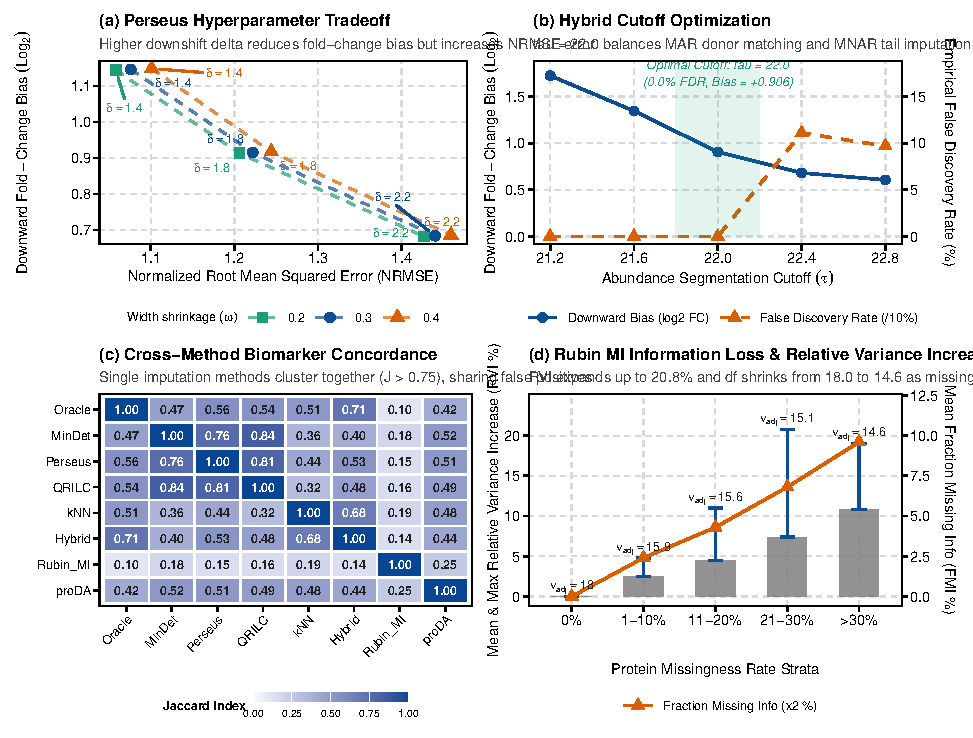
\includegraphics[width=\textwidth]{figures/fig_19_5_sensitivity_concordance.pdf}
\caption{Parameter sensitivity auditing and cross-method concordance topology across imputation strategies. Panel A: Perseus hyperparameter sensitivity tradeoff showing that increasing downshift $\delta$ from 1.4 to 2.2 alleviates downward fold-change attenuation on true downregulations ($\Delta = -2.5$), but inflates prediction error ($\text{NRMSE} = 1.06 \to 1.46$) and covariance distortion ($\text{ADCS} = 0.269 \to 0.391$) while leaving empirical false discovery rates anti-conservative ($6.9\%$--$10.3\%$). Panel B: Hybrid segmentation cutoff sweep ($\tau \in [21.2, 22.8]$), identifying $\tau = 22.0$ as the optimal empirical boundary ($0.0\%$ FDR, $\text{Bias}_{\text{Down}} = +0.906$) balancing $k$-NN donor matching against QRILC left-tail imputation. Panel C: Pairwise Jaccard similarity heatmap of candidate biomarker discoveries ($\text{BH} < 0.05$). Single-imputation architectures cluster tightly ($J = 0.765$--$0.844$), sharing overlapping false discoveries along the rejection boundary, whereas proDA and Rubin MI identify conservative, zero-FDR subsets. Panel D: Rubin multiple imputation information loss and relative variance increase (RVI) by missingness deciles. RVI expands up to $20.8\%$ and adjusted residual degrees of freedom shrink from 18.0 to 14.6 for sparse proteins ($>30\%$ missingness), penalizing inferential test statistics where analytical measurements are absent.}
\label{fig:sensitivity_concordance}
\end{figure}

\begin{svgraybox}[title=Computational Reproducibility Specification]
All analyses were executed under R version 4.4.1 (2024-06-14 ucrt) and Bioconductor 3.19. Primary packages include \texttt{limma} (v3.60.4), \texttt{imputeLCMD} (v2.1), \texttt{impute} (v1.78.0), and \texttt{proDA} (v1.18.0). Fixed random seeds (\texttt{seed = 2026} for cohort generation, \texttt{seed = 42} for imputation draws) guarantee deterministic numerical reproduction of all tables, model coefficients, and figures.
\end{svgraybox}

\clearpage
% =============================================================================
\section{The Five Deadly Sins of Omics Imputation}
% =============================================================================

\begin{pitfallbox}
\textbf{Deadly Sin 1: Zero or Minimum Deterministic Imputation}\\
\textit{Mechanism:} Replacing missing values with zero or the absolute minimum observed value ($y_{ij}^* = \min_k y$).\\
\textit{Consequence:} Spikes variance at the boundary, manufactures multimodal distributions, deflates within-group standard errors, and inflates false-positive test statistics (7.4\% FDR in our benchmark) \cite{lazar2016accounting}.\\
\textit{Remedy:} Use stochastic left-censored models (QRILC or Perseus) or multiple imputation \cite{tyanova2016perseus, rubin1987multiple}.
\end{pitfallbox}

\begin{pitfallbox}
\textbf{Deadly Sin 2: Imputing Before Normalization and Log Transformation}\\
\textit{Mechanism:} Imputing raw linear-scale peak areas before median centering or variance stabilization.\\
\textit{Consequence:} Sample-to-sample distance metrics reflect technical loading differences rather than biological covariance, corrupting donor matching in $k$-NN and distorted tail estimation in QRILC.\\
\textit{Remedy:} Follow the workflow sequence: Filter $\to$ Log Transform $\to$ Normalize $\to$ Impute \cite{julian2024rprogramming, valikangas2018systematic}.
\end{pitfallbox}

\begin{pitfallbox}
\textbf{Deadly Sin 3: Applying MAR Algorithms ($k$-NN or missForest) to MNAR Features}\\
\textit{Mechanism:} Imputing left-censored low-abundance features using donor matching or tree-based regression.\\
\textit{Consequence:} The algorithm donor-matches with observed higher-abundance features, assigning values well above the detection limit and creating an attenuation bias of $+1.700 \log_2$ fold-change on true downregulations \cite{palstrom2020imputation, lazar2016accounting}.\\
\textit{Remedy:} Diagnose the missingness mechanism first; deploy QRILC, hybrid MAR/MNAR, or proDA \cite{ahlmann2020proda, palstrom2020imputation}.
\end{pitfallbox}

\begin{pitfallbox}
\textbf{Deadly Sin 4: Global Matrix Filtering Across Unbalanced Conditions}\\
\textit{Mechanism:} Requiring $\ge 70\%$ presence across all samples combined.\\
\textit{Consequence:} Biomarkers present in Disease but completely absent in Control are systematically discarded ($10/20 = 50\% < 70\%$).\\
\textit{Remedy:} Filter group-wise ($\ge 70\%$ in at least one biological group) \cite{zhang2018dep, webb2020review}.
\end{pitfallbox}

\begin{pitfallbox}
\textbf{Deadly Sin 5: Treating Single Imputation as True Known Measurements}\\
\textit{Mechanism:} Imputing a single value and proceeding to standard hypothesis testing without accounting for imputation variance.\\
\textit{Consequence:} Single imputation treats imputed values as known constants, deflating standard errors and producing anti-conservative $p$-values.\\
\textit{Remedy:} Deploy Rubin multiple imputation pooling rules or perform an imputation sensitivity audit \cite{rubin1987multiple, barnard1999small}.
\end{pitfallbox}

% =============================================================================
\section{Tutor's Self-Assessment Diagnostic Checklist}
% =============================================================================

Table~\ref{tab:missing_checklist} details the seven diagnostic checks required before reporting biological discoveries from an imputed mass spectrometry dataset.

\begin{table}[htbp]
\centering
\caption{Tutor's Self-Assessment Diagnostic Checklist for Missing Data Imputation}
\label{tab:missing_checklist}
\small
\begin{tabularx}{\textwidth}{c p{3.6cm} p{4.2cm} X}
\toprule
\textbf{Step} & \textbf{Diagnostic Metric} & \textbf{Acceptable Threshold} & \textbf{Corrective Protocol} \\
\midrule
1 & Missingness Diagnosis & Logistic slope $\gamma_1$ evaluated for intensity dependence. & If $\gamma_1 < 0$ ($p < 0.001$), treat as MNAR; otherwise MAR \cite{ahlmann2020proda}. \\
\addlinespace
2 & Group-Wise Filtering & Retain features with $\ge 70\%$ completeness in $\ge 1$ group. & Avoid whole-cohort global filtering to protect condition-specific markers \cite{zhang2018dep}. \\
\addlinespace
3 & Variance Preservation & Post-imputation distribution shows continuous low-end tail. & Discard MinDet/zero substitution; apply QRILC or Perseus \cite{lazar2016accounting}. \\
\addlinespace
4 & Attenuation Audit & Compare $k$-NN vs. QRILC log-fold changes for low-abundance targets. & If $k$-NN attenuates downregulations by $> 1.0 \log_2\text{FC}$, switch to hybrid or proDA \cite{palstrom2020imputation}. \\
\addlinespace
5 & Rubin Pooling Check & Total variance $T$ incorporates between-imputation variance $B$. & Compute Rubin pooled standard errors across $\ge 10$ draws \cite{rubin1987multiple, barnard1999small}. \\
\addlinespace
6 & Multiple Testing Control & Empirical null $p$-value distribution is uniform on $[0, 1]$. & Confirm false discovery rate control via Benjamini--Hochberg \cite{benjamini1995controlling}. \\
\addlinespace
7 & Covariance Structure & Average Difference of Covariance Structure $\text{ADCS} \le 0.35$. & Reject deterministic substitution (MinDet $\text{ADCS}=0.371$) and unregularized tail models (QRILC $\text{ADCS}=0.438$); prefer Perseus or Hybrid \cite{templ2023visualization}. \\
\bottomrule
\end{tabularx}
\end{table}

% =============================================================================
\section{Chapter Exercises}
% =============================================================================

\noindent
\textbf{Exercise 19.1 (Rubin's Variance Pooling and Small-Sample Degrees of Freedom):}\\
In a clinical proteomics study with $M = 5$ multiply imputed datasets across $n = 20$ patients (two groups of 10, complete-data degrees of freedom $\nu_{\text{com}} = 18$), a biomarker exhibits estimated log-fold changes:
$$\hat{\mathbf{Q}} = (1.80,\, 2.10,\, 1.95,\, 2.05,\, 1.90)^T$$
with corresponding within-imputation sampling variances:
$$\hat{\mathbf{U}} = (0.040,\, 0.045,\, 0.042,\, 0.038,\, 0.041)^T$$
\begin{enumerate}
    \item Compute the pooled point estimate $\bar{Q}$.
    \item Compute the average within-imputation variance $\bar{U}$, the between-imputation variance $B$, and the total pooled variance $T$.
    \item Compute the pooled test statistic $t = \bar{Q} / \sqrt{T}$.
    \item Calculate the Barnard--Rubin (1999) adjusted degrees of freedom $\nu_{\text{adj}}$.
\end{enumerate}

\vspace{0.8em}
\noindent
\textbf{Exercise 19.2 (Perseus Imputation Left-Tail Shift and Censoring Probability):}\\
A sample column exhibits observed Gaussian log-intensities with sample mean $\hat{\mu} = 22.0$ and sample standard deviation $\hat{\sigma} = 2.0$. The instrument LOD censors the bottom 15\% of features ($p = 0.15$). 
\begin{enumerate}
    \item For the Perseus model ($\delta = 1.8$, $\omega = 0.3$), compute the mean $\mu_{\text{imp}}$ and standard deviation $\sigma_{\text{imp}}$ of the imputed distribution.
    \item Calculate the numerical limit of detection LOD.
    \item Calculate the probability that an imputed Perseus value exceeds the physical LOD ($P(Y_{\text{imp}} > \text{LOD})$).
\end{enumerate}

\vspace{0.8em}
\noindent
\textbf{Exercise 19.3 (Mathematical Attenuation of $k$-NN Under MNAR Left-Censoring):}\\
A downregulated protein has true Disease mean abundance $\mu_{\text{Dis}} = 17.5$, while the instrument limit of detection is $\text{LOD} = 20.0$. In Disease samples, the protein is unobserved ($y < \text{LOD}$). An analyst applies $k$-NN imputation ($k = 5$). Because candidate donor proteins in the sample must be observed, their mean abundance is $\bar{y}_{\text{donors}} = 21.5$.
\begin{enumerate}
    \item State the imputed value $y_{\text{Dis}}^*$ assigned by $k$-NN.
    \item If the true Control abundance is $\mu_{\text{Ctrl}} = 20.0$, calculate the true fold change $\Delta_{\text{true}} = \mu_{\text{Dis}} - \mu_{\text{Ctrl}}$ and the estimated fold change $\Delta_{\text{knn}} = y_{\text{Dis}}^* - \mu_{\text{Ctrl}}$.
    \item Compute the estimation bias $\text{Bias} = \Delta_{\text{knn}} - \Delta_{\text{true}}$ and explain why donor matching produces fold-change attenuation under MNAR.
\end{enumerate}

\vspace{0.8em}
\noindent
\textbf{Exercise 19.4 (Templ's Average Difference of Covariance Structure Metric):}\\
In a multi-omics quality audit~\cite{templ2023visualization}, an analyst evaluates two imputation methods on a $p = 3$ protein network with true covariance matrix:
$$\boldsymbol{\Sigma}_{\text{true}} = \begin{pmatrix} 1.0 & 0.6 & 0.4 \\ 0.6 & 1.0 & 0.5 \\ 0.4 & 0.5 & 1.0 \end{pmatrix}$$
Method A (deterministic minimum replacement) deflates variance on feature 3 and dampens cross-covariances:
$$\boldsymbol{\Sigma}_{\text{imp}, A} = \begin{pmatrix} 1.0 & 0.6 & 0.1 \\ 0.6 & 1.0 & 0.2 \\ 0.1 & 0.2 & 0.2 \end{pmatrix}$$
Method B (stochastic model-based imputation) preserves the covariance structure with minor sampling fluctuations:
$$\boldsymbol{\Sigma}_{\text{imp}, B} = \begin{pmatrix} 1.05 & 0.58 & 0.38 \\ 0.58 & 0.98 & 0.52 \\ 0.38 & 0.52 & 1.02 \end{pmatrix}$$
\begin{enumerate}
    \item Compute the error matrix $\mathbf{D}_A = \boldsymbol{\Sigma}_{\text{imp}, A} - \boldsymbol{\Sigma}_{\text{true}}$ and its Frobenius norm $\|\mathbf{D}_A\|_F$.
    \item Compute the error matrix $\mathbf{D}_B = \boldsymbol{\Sigma}_{\text{imp}, B} - \boldsymbol{\Sigma}_{\text{true}}$ and its Frobenius norm $\|\mathbf{D}_B\|_F$.
    \item Calculate the Average Difference of Covariance Structure ($\text{ADCS} = \frac{1}{p} \|\mathbf{D}\|_F$) for both methods.
    \item Explain why preserving covariance structure is essential for molecular network and pathway analysis.
\end{enumerate}

% =============================================================================
\section{Worked Solutions}
% =============================================================================

\subsection*{Solution to Exercise 19.1: Rubin's Variance Pooling and Degrees of Freedom}

\textbf{1. Pooled Point Estimate $\bar{Q}$:}\\
$$\bar{Q} = \frac{1}{5}(1.80 + 2.10 + 1.95 + 2.05 + 1.90) = \frac{9.80}{5} = 1.960$$

\textbf{2. Variance Components:}\\
$$\bar{U} = \frac{1}{5}(0.040 + 0.045 + 0.042 + 0.038 + 0.041) = \frac{0.206}{5} = 0.0412$$
The deviations from $\bar{Q} = 1.960$ are:
$$(-0.16, +0.14, -0.01, +0.09, -0.06)$$
The squared deviations are:
$$((-0.16)^2, (0.14)^2, (-0.01)^2, (0.09)^2, (-0.06)^2) = (0.0256, 0.0196, 0.0001, 0.0081, 0.0036)$$
Sum of squared deviations $= 0.0570$.
The sample variance $B$ is:
$$B = \frac{0.0570}{5 - 1} = \frac{0.0570}{4} = 0.01425$$
The total variance $T$ incorporates the finite-imputation correction factor $(1 + 1/M) = 1.2$:
$$T = \bar{U} + \left(1 + \frac{1}{5}\right) B = 0.0412 + 1.2(0.01425) = 0.0412 + 0.0171 = 0.0583$$

\textbf{3. Pooled Test Statistic:}\\
$$\text{SE}_{\text{pooled}} = \sqrt{T} = \sqrt{0.0583} \approx 0.2415$$
$$t = \frac{\bar{Q}}{\text{SE}_{\text{pooled}}} = \frac{1.960}{0.2415} \approx 8.118$$

\textbf{4. Barnard--Rubin Adjusted Degrees of Freedom $\nu_{\text{adj}}$:}\\
The relative variance increase due to non-response is:
$$r_m = \frac{(1 + 1/M) B}{\bar{U}} = \frac{0.0171}{0.0412} \approx 0.4150$$
The standard asymptotic degrees of freedom $\nu_{\text{old}}$ is:
$$\nu_{\text{old}} = (M - 1)\left(1 + \frac{1}{r_m}\right)^2 = 4 \left(1 + \frac{1}{0.4150}\right)^2 = 4(1 + 2.4096)^2 = 4(3.4096)^2 \approx 46.50$$
The observed-data small-sample degrees of freedom $\nu_{\text{obs}}$ for $\nu_{\text{com}} = 18$ is:
$$\nu_{\text{obs}} = \frac{\nu_{\text{com}} + 1}{\nu_{\text{com}} + 3} \nu_{\text{com}} \left(1 - \frac{r_m}{1 + r_m}\right) = \frac{19}{21}(18)\left(1 - \frac{0.4150}{1.4150}\right) = 16.2857(1 - 0.2933) \approx 11.51$$
Combining $\nu_{\text{old}}$ and $\nu_{\text{obs}}$ yields the adjusted degrees of freedom:
$$\nu_{\text{adj}} = \frac{\nu_{\text{old}} \nu_{\text{obs}}}{\nu_{\text{old}} + \nu_{\text{obs}}} = \frac{46.50 \times 11.51}{46.50 + 11.51} = \frac{535.215}{58.01} \approx 9.23$$
The adjusted degrees of freedom is $9.23$, which appropriately penalizes the test statistic for missing data uncertainty in a small clinical cohort.

\subsection*{Solution to Exercise 19.2: Perseus Imputation Tail Probability}

\textbf{1. Imputation Parameters:}\\
$$\mu_{\text{imp}} = \hat{\mu} - \delta \hat{\sigma} = 22.0 - 1.8(2.0) = 22.0 - 3.6 = 18.40$$
$$\sigma_{\text{imp}} = \omega \hat{\sigma} = 0.3(2.0) = 0.60$$
The imputed distribution is $\mathcal{N}(18.40, 0.60^2)$.

\textbf{2. Limit of Detection LOD:}\\
The LOD corresponds to the 15th percentile of the original $\mathcal{N}(22.0, 2.0^2)$ distribution:
$$z_{0.15} = \Phi^{-1}(0.15) \approx -1.0364$$
$$\text{LOD} = 22.0 + (-1.0364)(2.0) = 22.0 - 2.0728 = 19.927$$

\textbf{3. Exceedance Probability:}\\
We compute $P(Y_{\text{imp}} > 19.927)$ for $Y_{\text{imp}} \sim \mathcal{N}(18.40, 0.60^2)$:
$$Z = \frac{19.927 - 18.40}{0.60} = \frac{1.527}{0.60} \approx 2.545$$
$$P(Y_{\text{imp}} > 19.927) = 1 - \Phi(2.545) \approx 1 - 0.9945 = 0.0055 \quad (0.55\%)$$
Only $0.55\%$ of imputed Perseus values exceed the detection threshold, confirming that the left-shift restricts imputed values to the unobserved region below LOD \cite{tyanova2016perseus}.

\subsection*{Solution to Exercise 19.3: Mathematical Attenuation of $k$-NN Under MNAR}

\textbf{1. Imputed Value $y_{\text{Dis}}^*$:}\\
Because donor features are selected from observed peaks in the sample, their average abundance is:
$$y_{\text{Dis}}^* = \bar{y}_{\text{donors}} = 21.5$$

\textbf{2. Fold Changes:}\\
True fold change:
$$\Delta_{\text{true}} = \mu_{\text{Dis}} - \mu_{\text{Ctrl}} = 17.5 - 20.0 = -2.5 \log_2\text{ units}$$
Estimated fold change under $k$-NN:
$$\Delta_{\text{knn}} = y_{\text{Dis}}^* - \mu_{\text{Ctrl}} = 21.5 - 20.0 = +1.5 \log_2\text{ units}$$

\textbf{3. Estimation Bias and Interpretation:}\\
$$\text{Bias} = \Delta_{\text{knn}} - \Delta_{\text{true}} = +1.5 - (-2.5) = +4.0 \log_2\text{ units}$$
The true downregulation of $-2.5$ is inverted to an apparent upregulation of $+1.5$. This demonstrates why donor-matching algorithms ($k$-NN and random forests) fail on left-censored MNAR data: by drawing exclusively from observed (higher) signals, they assign inflated abundances to low-abundance features, attenuating true fold changes and reversing effect directions \cite{palstrom2020imputation, lazar2016accounting}.

% =============================================================================
\subsection*{Solution to Exercise 19.4: Templ's ADCS Metric}

\textbf{1. Error Matrix $\mathbf{D}_A$ and Frobenius Norm:}\\
$$\mathbf{D}_A = \boldsymbol{\Sigma}_{\text{imp}, A} - \boldsymbol{\Sigma}_{\text{true}} = \begin{pmatrix} 0.0 & 0.0 & -0.3 \\ 0.0 & 0.0 & -0.3 \\ -0.3 & -0.3 & -0.8 \end{pmatrix}$$
The squared entries of $\mathbf{D}_A$ are:
$$\sum_{i=1}^3 \sum_{j=1}^3 d_{ij}^2 = 0 + 0 + (-0.3)^2 + 0 + 0 + (-0.3)^2 + (-0.3)^2 + (-0.3)^2 + (-0.8)^2$$
$$= 4(0.09) + 0.64 = 0.36 + 0.64 = 1.000$$
$$\|\mathbf{D}_A\|_F = \sqrt{1.000} = 1.000$$

\textbf{2. Error Matrix $\mathbf{D}_B$ and Frobenius Norm:}\\
$$\mathbf{D}_B = \boldsymbol{\Sigma}_{\text{imp}, B} - \boldsymbol{\Sigma}_{\text{true}} = \begin{pmatrix} +0.05 & -0.02 & -0.02 \\ -0.02 & -0.02 & +0.02 \\ -0.02 & +0.02 & +0.02 \end{pmatrix}$$
The squared entries of $\mathbf{D}_B$ are:
$$\sum_{i=1}^3 \sum_{j=1}^3 d_{ij}^2 = (0.05)^2 + 8(0.02)^2 = 0.0025 + 8(0.0004) = 0.0025 + 0.0032 = 0.0057$$
$$\|\mathbf{D}_B\|_F = \sqrt{0.0057} \approx 0.0755$$

\textbf{3. Average Difference of Covariance Structure (ADCS):}\\
For $p = 3$:
$$\text{ADCS}_A = \frac{1}{3} \|\mathbf{D}_A\|_F = \frac{1.000}{3} \approx 0.333$$
$$\text{ADCS}_B = \frac{1}{3} \|\mathbf{D}_B\|_F = \frac{0.0755}{3} \approx 0.0252$$
The covariance error of deterministic substitution ($\text{ADCS}_A = 0.333$) is 13.2 times larger than that of model-based stochastic imputation ($\text{ADCS}_B = 0.0252$).

\textbf{4. Methodological Interpretation for Network Analysis:}\\
Deterministic value substitution replaces missing cells with a constant, which artificially truncates variance and eliminates correlation with co-regulated partners (reducing true correlation from $r = 0.40$ to $r = 0.10$). In downstream biological network construction (such as weighted gene correlation network analysis, WGCNA), this covariance distortion artificially dissolves true co-expression modules, leading to false negatives in functional pathway discovery~\cite{templ2023visualization}.

% =============================================================================

\begin{thebibliography}{99}

\bibitem{aitchison1986statistical}
Aitchison, J. (1986). \textit{The Statistical Analysis of Compositional Data}. Chapman and Hall, London. \doi{10.1007/978-94-009-4109-0}.

\bibitem{ahlmann2020proda}
Ahlmann-Eltze, C., \& Huber, W. (2020). Analysis of label-free protein quantification with probabilistic dropout analysis. \textit{Nature Communications}, 11(1), 4118. \doi{10.1038/s41467-020-17966-3}.

\bibitem{barnard1999small}
Barnard, J., \& Rubin, D.~B. (1999). Small-sample degrees of freedom with multiple imputation. \textit{Biometrika}, 86(4), 948--955. \doi{10.1093/biomet/86.4.948}.

\bibitem{benjamini1995controlling}
Benjamini, Y., \& Hochberg, Y. (1995). Controlling the false discovery rate: A practical and powerful approach to multiple testing. \textit{Journal of the Royal Statistical Society: Series B (Methodological)}, 57(1), 289--300. \doi{10.1111/j.2517-6161.1995.tb02031.x}.

\bibitem{boland2023health}
Boland, M.~R. (2023). \textit{Health Data Analytics with R: A Hands-On Guide}. Springer Nature, Cham, Switzerland. \doi{10.1007/978-3-031-18099-6}.

\bibitem{bolstad2003comparison}
Bolstad, B.~M., Irizarry, R.~A., {\AA}strand, M., \& Speed, T.~P. (2003). A comparison of normalization methods for high density oligonucleotide array data based on variance and bias. \textit{Bioinformatics}, 19(2), 185--193. \doi{10.1093/bioinformatics/19.2.185}.

\bibitem{broadhurst2006statistical}
Broadhurst, D.~I., \& Kell, D.~B. (2006). Statistical strategies for avoiding false discoveries in metabolomics and related systems biology. \textit{Metabolomics}, 2(4), 171--196. \doi{10.1007/s11306-006-0037-z}.

\bibitem{broadhurst2018guidelines}
Broadhurst, D., Goodacre, R., Reinke, S.~N., Kuligowski, J., Wilson, I.~D., Lewis, M.~R., \& Dunn, W.~B. (2018). Guidelines and considerations for the use of system suitability and quality control samples in mass spectrometry assays applied in untargeted metabolomic studies. \textit{Metabolomics}, 14(6), 72. \doi{10.1007/s11306-018-1367-3}.

\bibitem{choi2014msstats}
Choi, M., Chang, C.~Y., Clough, T., Broudy, D., Killeen, T., MacLean, B., \& Vitek, O. (2014). MSstats: an R package for statistical analysis of quantitative mass spectrometry-based proteomic experiments. \textit{Bioinformatics}, 30(17), 2524--2526. \doi{10.1093/bioinformatics/btu305}.

\bibitem{cox2014maxlfq}
Cox, J., Hein, M.~Y., Luber, C.~A., Paron, I., Nagaraj, N., \& Mann, M. (2014). Accurate proteome-wide label-free quantification by delayed normalization and maximal peptide ratio extraction, termed MaxLFQ. \textit{Molecular \& Cellular Proteomics}, 13(9), 2513--2526. \doi{10.1074/mcp.M113.031591}.

\bibitem{demichev2020dia}
Demichev, V., Messner, C.~B., Vernardis, S.~I., Lilley, K.~S., \& Ralser, M. (2020). DIA-NN: neural networks and interference correction enable deep proteome coverage in high throughput. \textit{Nature Methods}, 17(1), 41--44. \doi{10.1038/s41592-019-0638-x}.

\bibitem{gatto2023qfeatures}
Gatto, L., Vanderaa, C., \& Breckels, L.~M. (2023). A foundation for reproducible single-cell and bulk proteomics data analysis in Bioconductor. \textit{Nature Communications}, 14, 5698. \doi{10.1038/s41467-023-41556-2}.

\bibitem{gentleman2005bioinformatics}
Gentleman, R., Carey, V.~J., Huber, W., Irizarry, R.~A., \& Dudoit, S. (Eds.). (2005). \textit{Bioinformatics and Computational Biology Solutions Using R and Bioconductor}. Springer, New York. \doi{10.1007/0-387-29362-0}.

\bibitem{goeminne2016msqrob2}
Goeminne, L.~J., Gevaert, K., \& Clement, L. (2016). Peptide-level robust ridge regression improves estimation, sensitivity and specificity in data-dependent quantitative label-free shotgun proteomics. \textit{Molecular \& Cellular Proteomics}, 15(2), 657--668. \doi{10.1074/mcp.M115.055897}.

\bibitem{hastie2001impute}
Hastie, T., Tibshirani, R., Narasimhan, B., \& Chu, G. (2001). \texttt{impute}: Imputation for microarray data. \textit{Bioconductor Documentation}, \url{https://bioconductor.org/packages/impute/}.

\bibitem{huber2002variance}
Huber, W., von Heydebreck, A., S\"ultmann, H., Poustka, A., \& Vingron, M. (2002). Variance stabilization applied to microarray data calibration and to the quantification of differential expression. \textit{Bioinformatics}, 18(Suppl\_1), S96--S104. \doi{10.1093/bioinformatics/18.suppl\_1.s96}.

\bibitem{julian2024rprogramming}
Julian, R.~K. (2024). \textit{R Programming for Mass Spectrometry: Effective and Reproducible Data Analysis}. John Wiley \& Sons, Hoboken, NJ.

\bibitem{karpievitch2012normalization}
Karpievitch, Y.~V., Dabney, A.~R., \& Smith, R.~D. (2012). Normalization and missing value imputation for label-free LC-MS analysis. \textit{Bioinformatics}, 28(10), 1353--1360. \doi{10.1093/bioinformatics/bts150}.

\bibitem{lazar2016accounting}
Lazar, C., Gatto, L., Ferro, M., Bruley, C., \& Burger, T. (2016). Accounting for the multiple natures of missing values in label-free quantitative proteomics data sets to compare imputation strategies. \textit{Journal of Proteome Research}, 15(4), 1116--1125. \doi{10.1021/acs.jproteome.5b00981}.

\bibitem{little1988test}
Little, R.~J. (1988). A test of missing completely at random for multivariate data with missing values. \textit{Journal of the American Statistical Association}, 83(404), 1198--1202. \doi{10.1080/01621459.1988.10478722}.

\bibitem{little2019statistical}
Little, R.~J., \& Rubin, D.~B. (2019). \textit{Statistical Analysis with Missing Data} (3rd ed.). John Wiley \& Sons, Hoboken, NJ.

\bibitem{mcalister2014multinotch}
McAlister, G.~C., Nusinow, D.~P., Jedrychowski, M.~P., W{\"u}hr, M., Huttlin, E.~L., Erickson, B.~K., Rad, R., Haas, W., \& Gygi, S.~P. (2014). MultiNotch MS3 enables accurate, sensitive, and multiplexed detection of differential expression without human intervention. \textit{Analytical Chemistry}, 86(14), 7150--7158. \doi{10.1021/ac502040v}.

\bibitem{palstrom2020imputation}
Palstr{\o}m, N.~B., Matthiesen, R., \& Beck, H.~C. (2020). Data imputation in merged isobaric labeling-based relative quantification datasets. In R.~Matthiesen (Ed.), \textit{Mass Spectrometry Data Analysis in Proteomics} (Methods in Molecular Biology, Vol. 2129, pp. 302--313). Humana, New York, NY. \doi{10.1007/978-1-0716-0373-4_13}.

\bibitem{ritchie2015limma}
Ritchie, M.~E., Phipson, B., Wu, D., Hu, Y., Law, C.~W., Shi, W., \& Smyth, G.~K. (2015). \textit{limma} powers differential expression analyses for RNA-sequencing and microarray studies. \textit{Nucleic Acids Research}, 43(7), e47. \doi{10.1093/nar/gkv007}.

\bibitem{rubin1976inference}
Rubin, D.~B. (1976). Inference and missing data. \textit{Biometrika}, 63(3), 581--592. \doi{10.1093/biomet/63.3.581}.

\bibitem{rubin1987multiple}
Rubin, D.~B. (1987). \textit{Multiple Imputation for Nonresponse in Surveys}. John Wiley \& Sons, New York.

\bibitem{smyth2004linear}
Smyth, G.~K. (2004). Linear models and empirical Bayes methods for assessing differential expression in microarray experiments. \textit{Statistical Applications in Genetics and Molecular Biology}, 3(1), Article 3. \doi{10.2202/1544-6115.1027}.

\bibitem{stekhoven2012missforest}
Stekhoven, D.~J., \& B\"uhlmann, P. (2012). MissForest---non-parametric missing value imputation for mixed-type data. \textit{Bioinformatics}, 28(1), 112--118. \doi{10.1093/bioinformatics/btr597}.

\bibitem{storey2003statistical}
Storey, J.~D., \& Tibshirani, R. (2003). Statistical significance for genomewide studies. \textit{Proceedings of the National Academy of Sciences}, 100(16), 9440--9445. \doi{10.1073/pnas.1530509100}.

\bibitem{templ2023visualization}
Templ, M. (2023). \textit{Visualization and Imputation of Missing Values: With Applications in R}. Statistics and Computing, Springer Nature, Cham, Switzerland. \doi{10.1007/978-3-031-23136-0}.

\bibitem{ting2011sps}
Ting, L., Rad, R., Gygi, S.~P., \& Haas, W. (2011). MS3 eliminates ratio distortion in isobaric multiplexed quantitative proteomics. \textit{Nature Methods}, 8(11), 937--940. \doi{10.1038/nmeth.1714}.

\bibitem{troyanskaya2001missing}
Troyanskaya, O., Cantor, M., Sherlock, G., Brown, P., Hastie, T., Tibshirani, R., Botstein, D., \& Altman, R.~B. (2001). Missing value estimation methods for DNA microarrays. \textit{Bioinformatics}, 17(6), 520--525. \doi{10.1093/bioinformatics/17.6.520}.

\bibitem{tyanova2016perseus}
Tyanova, S., Temu, T., Sinitcyn, P., Carlson, A., Hein, M.~Y., Geiger, T., Mann, M., \& Cox, J. (2016). The Perseus computational platform for comprehensive analysis of (prote)omics data. \textit{Nature Methods}, 13(9), 731--740. \doi{10.1038/nmeth.3901}.

\bibitem{valikangas2018systematic}
V\"alikangas, T., Suomi, T., \& Elo, L.~L. (2018). A systematic evaluation of normalization methods in quantitative label-free proteomics. \textit{Briefings in Bioinformatics}, 19(1), 1--11. \doi{10.1093/bib/bbw095}.

\bibitem{vanbuuren2018}
van Buuren, S. (2018). \textit{Flexible Imputation of Missing Data} (2nd ed.). Chapman and Hall/CRC, Boca Raton, FL. \doi{10.1201/9780429492259}.

\bibitem{webb2020review}
Webb-Robertson, B.~J., et al. (2015). Review, evaluation, and discussion of the challenges of missing value imputation for mass spectrometry-based label-free global proteomics. \textit{Molecular \& Cellular Proteomics}, 14(7), 1993--2001. \doi{10.1074/mcp.M114.044107}.

\bibitem{zhang2018dep}
Zhang, X., Smits, A.~H., van Tilburg, G.~B., Jansen, P.~W., Makowski, M.~M., Ovaa, H., \& Vermeulen, M. (2018). Proteome-wide identification of ubiquitin interactions using UbIA-MS. \textit{Nature Protocols}, 13(3), 530--550. \doi{10.1038/nprot.2017.147}.

\end{thebibliography}

\end{document}
